\documentclass[twoside,11pt,ShortChapTitles]{BYUTextbook}

\usepackage{soul}
\renewcommand{\vec}[1]{\ensuremath{\mathbf{#1}}}
\usepackage{siunitx}
\sisetup{round-mode = figures,
  round-precision = 3, scientific-notation=true}

\begin{document}

\frontmatter

 \thispagestyle{empty}
 \begin{adjustwidth}{}{-1.5in}
 \centering
 {\huge INTRODUCTION TO PYTHON}
 \vskip1.5truein

    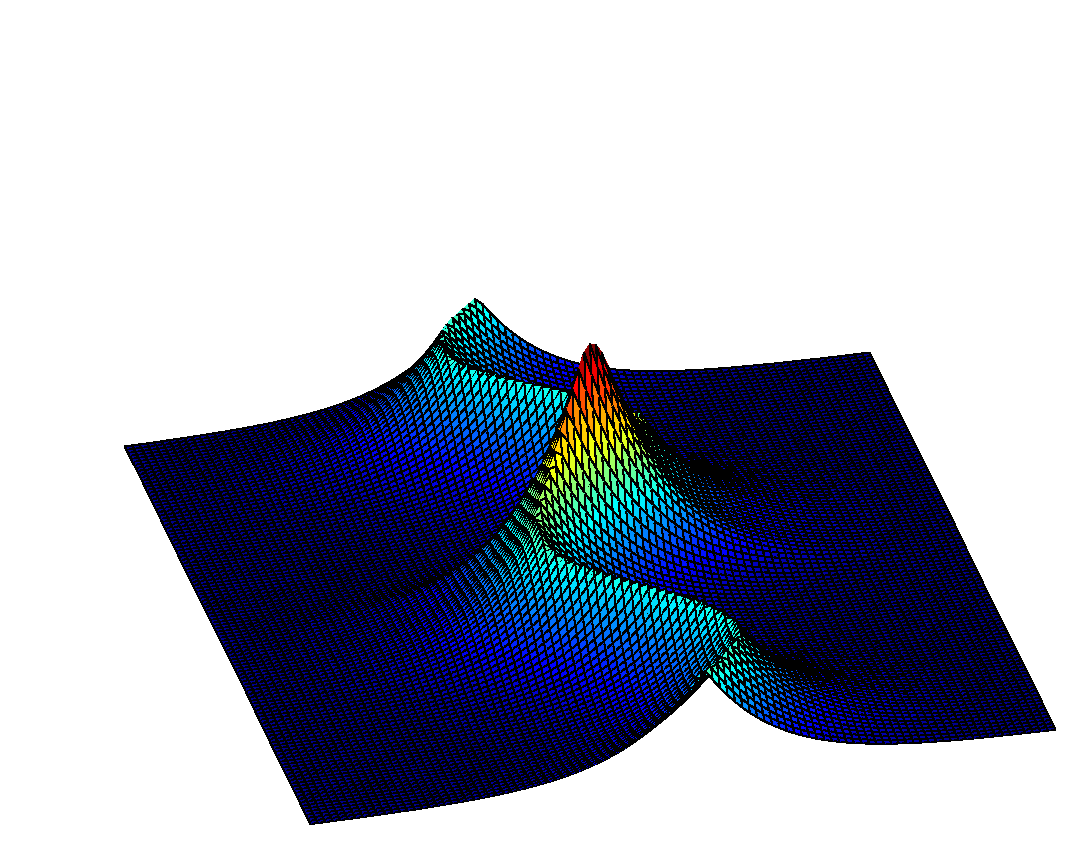
\includegraphics[scale=.80]{matlabcover}

\vskip1truein
Lance J.\ Nelson and Matthew R. Zachreson

\vskip.4truein
Department of Physics
\end{adjustwidth}

\cleardoublepage
\thispagestyle{empty}

 \begin{adjustwidth}{}{-1.5in}
 \centering
 \vspace*{1in}
 \large
 {\huge INTRODUCTION TO PYTHON}
 \vskip.4truein

 Lance J.\ Nelson and Matthew R. Zachreson
 \bigskip

 Department of Physics

 \bigskip
 Brigham Young University--Idaho

 \vfill


 {\footnotesize $\copyright$ 2017 Lance J.\ Nelson and Matthew R. Zachreson
               Brigham Young University--Idaho}

 \vskip.5truein
 {\footnotesize \emph{Last Revised: \today}}
 \normalsize

 \end{adjustwidth}

\cleardoublepage

\chapter*{Preface}

This is a tutorial to help you get started in Python.  This is a book for beginners. It assumes that you have no programming experience at all.

Examples of Python code in this book are in font \code{like
this}. As you read through the text, type and execute in Python all
of the examples. Longer sections of code
are set off and named.

There are three major parts to this book: {\em Preliminaries}, {\em The Basics}, and {\em Advanced Topics}.

{\em Preliminaries} walks you through how to get Python installed and running, and then gives tips on what to do when your programs don't work.

We designed {\em The Basics} section to teach you Python, piece by piece.  Each chapter builds on the last, and teaches you something new. You should work through each chapter, one by one, in order.

{\em Advanced Topics} covers things that are very useful in Python, but it serves more as a reference guide.  Go through the chapters there either when you need to use what is in them, or if you just want to learn something new.  Each chapter works as a stand alone tutorial, assuming that you've already covered {\em The Basics}.

In addition to teaching you Python, this booklet can also be used as a reference manual because it is
short and has lots of examples.

 Please tell us about mistakes and make suggestions to improve the text
(nelsonla@byui.edu).




 \cleardoublepage \phantomsection
 \addcontentsline{toc}{chapter}{Table of Contents}
\tableofcontents

\mainmatter
\part{Getting Started}
\chapter{Running Python}
\label{chap:RunningPython}

\marginfig{Figures/PythonCW.jpg}{Canopy's environment for running
  Python code.}

Python is a computer programming language (don't freak out) with broad
applicability in science and engineering.  For those that are brand
new to computer programming, Python is simply a way to communicate a
set of instructions to your computer.  You'll quickly learn that your
computer is great at doing exactly what you tell it to do.  If you
find that your computer isn't doing what you think it should, it is
not because the machine is malfunctioning, rather you just probably
don't fully understand what you are telling it to do.

There are two ways to run Python. One is at the command line\sidenote{If you are already comfortable with command line, then you probably don't need any help getting started. Feel free to use whatever editor you'd like. You'll need to make sure that you have Python 3 installed along with the following packages: numpy, scipy, matplotlib, iPython, sympy, and nose. These packages come pre-bundled with the Canopy distribution of Python, so if you installed Canopy, you already have them.} and the
other is through an IDE (integrated development environment). If you
don't know what the command line is, I recommend you start out using
an IDE. A good IDE for Python is called Canopy, which can
be downloaded \href{https://store.enthought.com/downloads/}{here}. This text is written for Python 3, so choose the Python 3.x download that matches your operating system (Windows, Mac, or Linux).


\section{Running Your First Program}

Once you have downloaded and installed Canopy, launch the editor. You should see a window that looks similar to the one displayed in the margin. (You may have to choose "Create a new file".) The Canopy Editor has three main windows: The file browser, the editor itself, and the Python console (Labeled "Python").
The file browser shows your local file directory.  It is nice to have when you write larger Python programs. To keep big programs easy to read, we often break them into several files.
The editor itself will be where we write our Python programs. We'll address the Python Console in a moment. Right now, type

\begin{Verbatim}
print('Hello World')
\end{Verbatim}

into the editor. Save your program as \code{myFirstProgram.py}, then click the green
arrow above the editor. If you look down at the console it should say:

\begin{Verbatim}
%run "where you saved the file/myFirstProgram.py"
Hello World
\end{Verbatim}
(If you don't see the words "Hello World", double check that what you've written in the editor and matches the above code exactly.) Congratulations, you just ran your first Python program. You told the computer to write "Hello World" on the console.
Now try changing this line:
\begin{Verbatim}
print('Hello World')
\end{Verbatim}
to this:
\begin{Verbatim}
print('I can do Python!')
\end{Verbatim}
and run your program again.\sidenote{You only need to do a "save as" on new files. Once you've given it a filename, Canopy will save and run your file every time you click the green arrow button.}
\section{The Python Console}
The Python console serves two purposes: First, it shows our program's outputs. (The "Hello World" from earlier.) Second, it allows us to do interactive Python. Try typing
\begin{Verbatim}
print('Hello World')
\end{Verbatim}
directly into the console, then press enter.  You should see it print
\code{Hello World}, just like it did for your program. The console
will run any Python command that you enter into it. It can be very
useful for short, quick calculations, or for looking at data when you
are trying to figure out what your program is doing. However, it is
impossible to save the commands that you enter into the console, so
you should do most of your programming in the editor.


\section{It's a Calculator}
The very easiest, yet meaningful thing you can with Python is to
perform simple math. Simple math can be performed pretty much just as
you would expect. Here are a few examples\sidenote{The \code{#} marks something called a comment.  Python knows to ignore anything on a line that comes after a \code{#}.  They exist so that you can leave notes to anyone reading the program, without affecting what the program does.}
\begin{Verbatim}
print(1+2)
print(5.0/6.0)
print(5**6)  # 5 raised to the power 6
print(678 * (3.5 + 2.8)**3.)
\end{Verbatim}
Note that typing the calculation alone, without the \code{print}
statement, will not produce any output to the screen.  Even though the
calculation has been performed, you will not see the result unless you
\code{print} it. Throughout this book, the \code{print}
statement will usually be omitted in code examples to maintain
brevity.  You should always print your result so you can see what you
have done.

\chapter[Debugging]{Debugging - Fixing Broken Code}
\label{chap:debug}

This chapter is a little different from the others.  The rest of this book is designed for you to read through and write Python as you go.  This chapter gives you some tips and tricks on finding mistakes in your code, but it isn't very useful until you have some.
We put this chapter at the beginning of the book so that you, the reader, would know it is here, and know to come back to it when you get stuck.

Skip this chapter.  Go on to the next one.  Come back when one of your programs starts spitting out error messages that you don't understand, or when it isn't doing what you think it should. That's when this chapter will be helpful.

\section{What is a Bug?}

In programming, we refer to any mistakes in your code as a "bug". The term "bug" also refers to anytime your code does something that you don't expect it to.  As a programmer, you will be spending a good amount of your time trying to find and fix these bugs.  We call that "debugging".

All programmers make mistakes, even the experts.  Making bugs is such a common occurrence that it's often said, "the only bug free code is no code at all."

 Bugs generally come in two types: ones that break your code and ones that don't do what you think.


\section{Bugs That Break Your Code - Error Messages}
As Python reads through your program, if it reaches a line of code that it can't read, or doesn't know what to do with, it will stop and print out an error message.  The message that it prints out is intended to help you, so you should learn to read it.

Here's an example of an error message:
\begin{Verbatim}
Traceback (most recent call last):
  File "errorExample.py", line 136, in <module>
    calculated_var=my_func(x,y)
  File "errorExample.py", line 63, in my_func
    divisor=int(xx/y)
NameError: name 'xx' is not defined
\end{Verbatim}
Let's break it down, piece by piece, starting with:
\begin{Verbatim}
Traceback (most recent call last):
\end{Verbatim}
This lines tells you that Python is going show you the steps that led up to the error, or trace back to it.  The next several lines show you those steps.  Here's the first place Python noticed the problem:
\begin{Verbatim}
  File "errorExample.py", line 136, in <module>
    calculated_var=my_func(x,y)
\end{Verbatim}
This tells me that in my file \code{errorExample.py}, something went wrong when Python tried to execute the command \code{calculated_var=my_func(x,y)}.  The next set of lines tells me that the problem is in the function \code{my_func}:
\begin{Verbatim}
  File "errorExample.py", line 63, in my_func
    divisor=int(xx/y)
\end{Verbatim}
Specifically, something went wrong on line 63, in the file \code{errorExample.py}. Line 63 contains the code \code{divisor=int(xx/y)}.

The last line of the error statement tells me what I did wrong:
\begin{Verbatim}
NameError: name 'xx' is not defined
\end{Verbatim}
I used a variable \code{xx} without defining it first. The \code{NameError:} at the beginning tells me what kind of mistake I made, then the \code{name 'xx' is not defined} gives more details about the problem.  Here are the different types of errors that you can get, along with ideas on things you should try to fix them.

\subsection*{AttributeError}
Attribute errors occur when you try to use a method (one of the \code{.} functions) that doesn't exist.  For example,  if you set \code{x=5}, then \code{x.append(7)} will create an attribute error, since you can't \code{append} to an integer.

You will also get this error if you misspell the method.  Even if \code{y} is a list, \code{y.appned(5)} will create an error because \code{appned} isn't a method.  \code{y.append(5)} will work just fine.

\subsection*{SyntaxError}
Syntax errors occur when you've made a mistake formatting your code.  Check these sorts of things:
\begin{itemize}
\item You've forgotten a \code{:} at the end of a \code{def}/\code{if}\code{for}\code{while} line.
\item You've forgotten to put quotes around a string, or you've mismatched the type of quotes.
\item You have mismatched brackets or parentheses.
\end{itemize}
The parenthesis can be a little harder to track down, because Python will tell you the line number where it noticed there was a problem with parentheses.  Since Python also uses parentheses to break one long line of code into multiple lines, the mismatch might be earlier in your program.

\subsection*{NameError}
Name errors occur whenever Python doesn't recognize the name of a variable or a function.  Here are some common reasons:
\begin{itemize}
\item You misspelled the variable/function/method namem
\item You use a function from a package that you forgot to import
\item You forgot to define a variable
\item You use a function before you define it
\item You forgot to put quotes around a string so Python is trying to read it as a variable.
\end{itemize}

\subsection*{TypeError}
Type errors occur whenever you try to do an opperation on the wrong data type.  You can't do float operations on a list, for example.  Nor can you divide by a string.

Here's an example of the most common type error I see from beginning programmers:
\begin{Verbatim}
v=[5.0, 6.0, 7.5]
t=5.0
x=v*t
\end{Verbatim}
Python does not know how to multiply a list (\code{v}) by a float (\code{t}), so (\code{v*t}) gives a type error.

However, this code will run fine:
\begin{Verbatim}
v=[5.0, 6.0, 7.5]
t=5.0
x=v[1]*t
\end{Verbatim}
since \code{v[1]} is \code{6.0} (a float), Python has no problem multiplying \code{5.0*6.0}.

\subsection*{IndentationError}
Python uses indentation to figure out when functions and loops begin and end.  If you have too many spaces, (or too few) you will get an indentation error.

You also aren't allowed to mix tabs and spaces.  Even if two rows look like they are lined up, if one was indented with a tab and the other with a few spaces, you will get an indentation error.  If you are using Canopy, you probably won't run into this problem. Every time you use tab to indent, Canopy automatically replaces tab with four spaces.

There are a few other types of errors that you may run into, but these are the most common.  If you are ever completely stumped by an error message, you can usually find answers by just copying the error type and details (the stuff after the \code{:}) and searching for it on Google.

\subsection*{Errors When Using Imported Packages}
If you've imported a package like Numpy, and give the wrong thing to one of the Numpy functions, you will get a very long error message that lists every function that the Numpy function you used depends on.  Here's an example:

\begin{Verbatim}
Traceback (most recent call last):
  File "errorExample.py", line 4, in <module>
    plt.plot(data,y)
  File "/Users/test_usr/canopy/lib/Python3.4/site-packages/matplotlib/...
       pyplot.py",  line 3099, in plot
    ret = ax.plot(*args, **kwargs)
  File "/Users/test_usr/canopy/lib/Python3.4/site-packages/matplotlib/...
       axes/_axes.py",  line 1373, in plot
    for line in self._get_lines(*args, **kwargs):
  File "/Users/test_usr/canopy/lib/Python3.4/site-packages/matplotlib/...
       axes/_base.py",  line 304, in _grab_next_args
    for seg in self._plot_args(remaining, kwargs):
  File "/Users/test_usr/canopy/lib/Python3.4/site-packages/matplotlib/...
       axes/_base.py",  line 282, in _plot_args
    x, y = self._xy_from_xy(x, y)
  File "/Users/test_usr/canopy/lib/Python3.4/site-packages/matplotlib/...
       axes/_base.py",  line 223, in _xy_from_xy
    raise ValueError("x and y must have same first dimension")
ValueError: x and y must have same first dimension
\end{Verbatim}

When that happens, the most useful thing to do is start at the top of the traceback and find the last time that it says the error is in your program.  Then, read the error at the bottom.  Here are the relevant bits of that long error message:

\begin{Verbatim}
Traceback (most recent call last):
  File "errorExample.py", line 4, in <module>
    plt.plot(data,y)
ValueError: x and y must have same first dimension
\end{Verbatim}
This lets me know that there is something wrong with my plot command on line 4. The \code{must have the same first dimension} part of the error lets me know that there is something wrong with the sizes of \code{data} and \code{y}.

\section{Bugs that don't make errors}
As you practice programming in Python, you will start to make fewer and fewer mistakes that Python will catch.  Your program will run without any errors, but it doesn't do what you expect it to.

When that happens, it tells you that you've written your Python perfectly, but you've told your computer to do the wrong thing.  For example, a plot might not have the right axes or
you might calculate a distance that is three times further than what you expected.

To catch these sorts of bugs, hunt for them with a bottom-up approach\sidenote{If you have a very large program with lots of pieces, sometimes it can be faster to do a top-down approach to find out which piece is broken, then do a bottom-up approach on just that piece.}.  Start at place furthest down in your code where you know something has gone wrong.  If you are having a problem with a plot, first check the plot commands themselves to see if everything is in order.

If everything looks ok in your plot command, check the variables that you are plotting.  If you have a problem with the command
\begin{Verbatim}
plt.plot(x,y)
\end{Verbatim}

Tell your program to print \code{x} and \code{y} just before you try to plot them:
\begin{Verbatim}
print(x)
print(y)
plt.plot(x,y)

\end{Verbatim}
then run your program again. When they print\sidenote{You can also see what is stored in the variable \code{x} by typing \code{x} into the console and hitting enter.}, check and see if \code{x} and \code{y} have the sort of information in them that you expect.  If they don't, look back at the part of the program where you made \code{x} and \code{y}, then continue looking backwards until you find your mistake.

\section{Toy Problems}
Often times when we write programs that do calculations for us, we test them out with toy problems.  For example, if you write a program that fits a line to some data, you can test it out by giving it data where you already know the slope and intercept.  If you set
\begin{Verbatim}
x=[0,1,2,3,4,5]
y=[0,1,2,3,4,5]
\end{Verbatim}
Your line fitting function should return a slope of \code{1.0} and an intercept of \code{0.0}. If it doesn't, you definitely know that you've done something wrong.

As another example, if you are writing a program that will calculate the path a projectile will take when fired through the air while including air resistance, first leave out air resistance and see if your program will match what you expect from kinematics.

Toy problems won't help you catch all of your bugs, but they are a quick and easy way to catch many of them.



\part{The Basics}
\chapter{Variables and Data Types}
\label{chap:variablesDataTypes}

When writing a computer program, there are several big ideas, or main
pillars, that you should grasp to be successful.  Two of those pillars
are variables and functions. This chapter will focus on assigning,
manipulating, and using different variable types.  Later chapters will
focus on other main ideas and some more specific tasks that can be
accomplished using these foundational ideas.

The simplest, and most fundamental object when programming a computer
is the variable, which is nothing more than a name which is given to a
piece of information. It allows the information to be saved (stored)
so that it can be recalled and used later.  \index{Data types} There
are different types of variables and each has it's use and
limitations.  Python has many types of variables, but you will mostly
use the following types: integers, floats, lists, and arrays.  What
follows is a brief description of each variable type (we'll save our
discussion of arrays until later) with some examples to illustrate.

\section{Integer variables}
Some of you may be used to programming in C++\sidenote{C++ is a
  compiled language, whereas Python is an interpreted language}, where
the variables are declared before a value is assigned.  In python,
variables are created and assigned in one statement using the
assignment operator (\code{=}).  The simplest type of data is an
integer, a decimal-less number.  An integer variable is created and
assigned a value like this:\index{Assigning values}
\begin{Verbatim}
a = 20
\end{Verbatim}
This statement creates the variable \code{a} and assigns it a value of
$20$ (an \textbf{integer}).  The value of \code{a} can be modified in
any way you choose.  For instance, the statement
\begin{Verbatim}
a = a + 1
\end{Verbatim}
adds one to whatever value was previously stored in
\code{a}. \sidenote{An assign statement in programming is not a
  mathematical equation.  It makes perfect sense to write
  \code{a=a+1} as assign statement: it tells the computer to get the
  value of \code{a} and add 1 to it and then store the evaluated
  quantity back in the variable \code{a}.  However, the mathematical
  equation $a=a+1$ is clearly false.}  Note that {\it variable names
  in Python are case sensitive,} so watch your capitalization.
\index{Case sensitive}
You can define multiple variables by putting the assignements on
seperate lines:
\begin{Verbatim}
a = 2
b = 4
c = a * b
\end{Verbatim}
Here we have stored the value $2$ in \code{a}, the value $4$ in
\code{b} and then used those assignments to calculate a new value: $ 2
\times 4$ and assign that value to the variable \code{c}.
%\reminder{\lefthand}{If you are using version 3 or higher of python,
%  printing a variable is done like this: \code{print(a)}.}
Other common mathematical operations can be performed on integer
variables.  For example:
\begin{Verbatim}
a = 20
b = 15
c = a + b  # add two numbers
d = a/b    # divide two numbers
r = a//b   # return only the quotient(an integer) of the division
r = a % b   # return only the remainder(an integer) of the division
e = a * b  # multiply two numbers together
f = c**4   # raise number to a power (use **, not ^)
\end{Verbatim}
Notice that performing an operation on two integers \ul{usually}
yields another integer.  The one exception is division if you are
using Python version 2 or earlier.  This can pose a serious problem if
you think about it for a second.  For example, what would be the value
of \code{d} above if the result has to be an integer?

\section{Float variables}
Most meaningful calculations should be performed using floating point
numbers, or floats in Python.  Float variables are created and assigned
in
one of two ways.  The first way is to simply include a decimal place
in the number, like this
\begin{Verbatim}
a = 20.
\end{Verbatim}
You can also cast an integer variable to a float variable using the
\code{float} command
\begin{Verbatim}
a = 20
b = float(a)
\end{Verbatim}
You may wonder what would happen when a float and an integer are used
in a calculation, like this
\begin{Verbatim}
a = 0.1
b = 3 * a  #Integer multiplied by a float results in a float.
\end{Verbatim}
\marginpar{\footnotesize\captionsetup{type=table}
  \vspace{-2.5in}
\begin{tabular}{lp{1.05in}}
\code{abs(x)} & Find the absolute value of x\\ \\
\code{divmod(x,y)}        & Returns the quotient and remainder when
using long division.\\ \\
\code{x \% y}      & Return the remainder of $\frac{x}{y}$ \\ \\
\code{float(x)}      & convert \code{x} to a float. \\ \\
\code{int(x)}      & convert \code{x} to an integer. \\ \\
\code{round(x)}  & Round the number \code{x} using standard
rounding rules \\ \\
\end{tabular}
\captionof{table}{A sampling of built-in functions commonly used with
integers
  and floats.\label{tab:HousekeepingFloats}}
}.
The result of such a calculation is always a float.  Only when
all of the numbers used in a calculation are integers is the result an
integer.
Floats can be entered using scientific notation like this
\begin{Verbatim}
1.23e15
\end{Verbatim}

\section{Boolean variables}
A boolean variable is one that stores one of two possible values: True
or False.  A boolean variable is created and assigned similar to the
other variables you've studied so far
\begin{Verbatim}
myVar = True
\end{Verbatim}
The purpose for using a boolean variable will become more clear as you
study loops and logical statements, so stay tuned.

\section{Lists}
It is very important that you fully grasp the concept of a list
variable.  They are heavily-used in mathematical and scientific
programming.  You can think of a list as a container that holds
multiple pieces of information. The list could hold integers, floats,
strings, or really just about anything.  Let's see how we might create
a list.

\subsection*{Creating Lists}
The easiest way to create  a list is by putting the list element
inside of square brackets, like this:
\begin{Verbatim}
a = [5.6 , 2.1 , 3.4 , 2.9]
\end{Verbatim}
Note that square brackets (\code{[]}) must be used when creating the
list. If you accidentally use parenthesis (\code{()})\sidenote{Use
  parenthesis to create a tuple, which is just like a list but cannot
  be modified.}  or curly brackets (\code{\{\}})\sidenote{Use curly
  brackets to create a dictionary, which is like a list but can be
  indexed on any data type, not just integers} you'll end up creating
something other than a list.
Another way to create a list is with
Python's \code{range} function:
\begin{Verbatim}
a = range(10,52,3)
\end{Verbatim}
This will construct a list of \ul{integers} starting at $10$, ending at
$52$, while stepping in increments of $3$. This function can also be
called with $1$ or $2$ arguments and default values will be assigned
to the missing ones.
\begin{Verbatim}
a = range(3,9)  # Creates a list starting at 3, ending a 9 stepping
                # in increments of 1 (default value)
b = range(10)   # Creates a list starting at 0(default), ending at 10
stepping
                # in increments of 1(default value)
\end{Verbatim}
\noindent You can make a list of anything.  For example, here is a
list of strings:
\begin{Verbatim}
a = ['Physics' , 'is' , 'so' , 'great']
\end{Verbatim}
The individual elements of any list need not be the same type of
data.  For instance, the following list is perfectly valid
\begin{Verbatim}
# Here is a list of strings and integers
a = ['Ben',90,'Chad',75,'Andrew',22]
\end{Verbatim}
You can even define a list of lists:
\begin{Verbatim}
a = [[4,3,2],[1,2.5,90],[4.2,2.9,10.5],[239.4,1.4],[2.27,98,234,16.2]]
\end{Verbatim}
\subsection*{Accessing and Slicing lists}
Accessing an element of a list (this will be done frequently so pay
attention!) can be accomplished using square brackets, like this
\begin{Verbatim}
a[0]  # Access the 1st element of array a
a[4]  # Access the 5th element of array a
a[-1] # Access the last element of array a
a[-2]  # Access the second to last element of array a
\end{Verbatim}
Take special note to the last two statements where a negative index is
used.  Using a negative index means that you are counting from the
back of the list forward.
Please note that python lists are zero-indexed: the first element of
any list is 0, the second element is 1, etc.  Lists can be easily
modified by specifying which element you want to change and what you
want it changed to:
\begin{Verbatim}
a = ['Physics' , 'is' , 'so' , 'great']
a[3] = 'tough'  # Change the 4th element of a to "tough"
\end{Verbatim}
At times you may want to access entire sections of list, though not
the entire list.  You can do this with the \code{:} operator, like
this
\begin{Verbatim}
aList = [4,5,10,1560,23,19]
aList[1:]
aList[1:3]
aList[:3]
aList[1:4:2]
\end{Verbatim}
There can be three numbers inside the brackets, each seperated by the
\code{:} symbol, like this \code{[x:y:z]}.  The section of the
list that is extracted starts at element \code{x}, ends at element
\code{y} (but does not include element \code{y}), while stepping in
increments of \code{z}.  Note that the last number is optional, and
omitting it will result in a default value of 1 for the step size.


When working with a list of list (also called a 2-dimensional list)
accessing an individual element requires two indices, like this
\begin{Verbatim}
a = [[4,3,2],[1,2.5,90],[4.2,2.9,10.5],[239.4,1.4],[2.27,98,234,16.2]]
c = a[3][1]
\end{Verbatim}
Here \code{[3][1]} means we are accessing the 2nd element of the 4th
list. (remember: Python lists are zero-indexed)
 \marginpar{\footnotesize\captionsetup{type=table}
  \vspace{-4.5in}
\begin{tabular}{lp{1.05in}}
\code{a[x]}        & Access element \code{x} in list \code{a}\\
\code{a[x:y:z]}        & Extract a slice of list \code{a}\\
\code{a.append(x)}        & Append \code{x} to list \code{a} \\
\code{a.pop()}      & Remove the last element of list \code{a}. \\
\code{len(a)}  & Find the number of elements in \code{a} \\
\code{range(x,y,z)}  & Create a list of integers, starting at x,
ending at y, and stepping in increments of z.\\
\code{a.insert(x,y)}    & Insert \code{y} at location
\code{x} in list \code{a} \\
\code{a.sort()}  & Sort list \code{a} from least to greatest. \\
\code{filter(f,x)}        & Filter list \code{x} using the
criteria function \code{f}(see lambda functions).\\
\code{a.reverse()}  & Reverse the order of list \code{a}. \\
\code{a.index(x)}  & Find the index where element x resides. \\
\code{a + b}  & Join list \code{a} to list \code{b} to form one
list. \\ \\
\code{max(a)}  & Find the largest element of \code{a} \\ \\
\code{min(a)}  & Find the smallest element of \code{a} \\ \\
\code{sum(a)}  & Returns the sum of the elements of \code{a} \\ \\
\end{tabular}
\captionof{table}{A sampling of ``housekeeping'' functions for
lists.\label{tab:HousekeepingList}}
}
\subsection*{Built-in Functions for Lists}
Python has many built-in functions that work on lists.  You've already
seem some of them.  Here are a few examples
\begin{Verbatim}
myList = range(5,25,2)  # Create list starting at 5, ending at 25,
                        # in increments of 2
len(myList)             # Find how many elements are in myList
myList.append(520)      # Add the number 520 to the end of myList
\end{Verbatim}
 Here, \code{range} will create a list \underline{of integers }
starting at $5$, ending at $25$ in increments of $2$.  The
\code{len} function will find the length of a list, and
\code{append} will add an element to the end of a list.  Table
\ref{tab:HousekeepingList} lists some of the more common built-in
functions/operations for lists.  Please note that this is not a
comprehensive list.  A complete list of available function can be
found in the appendix.


\subsection*{A warning: What not to do with lists}
There are several things that seem natural to do with lists but that
should not (cannot) be done.  First, it may be tempting to associate a
2-D list with a matrix and try to use the \code{:} to slice out a
submatrix.  For example, what if you defined the following 2D list
\begin{Verbatim}
from numpy import array
a = array([[1,2,3],[4,5,6],[7,8,9]])
\end{Verbatim}
and interpreted it as this matrix:
\begin{equation}
\left( \begin{tabular}{ccc}
1 & 2 & 3\\
4 & 5 & 6\\
7 & 8 & 9\\
\end{tabular}
\right)
\end{equation}
If you wanted to slice out the following 2 x 2 sub-matrix:
\begin{equation}
\left(\begin{tabular}{cc}
5 & 6 \\
8 & 8 \\
\end{tabular}
\right)
\end{equation}
and you tried to do it like this:
\begin{Verbatim}
b[1:3][1:3]
\end{Verbatim}
you would be disappointed to find out that it did not work.  Lesson
\#1: Don't treat 2D lists as matrices.

Second, you may feel tempted to associate a list with a mathematical
vector and try to perform vector math on them. For instance, it may
seem natural to try
\begin{Verbatim}
a = [5.1 , 3.2 , 6.8 , 9.2]
b = 5 * a
\end{Verbatim}
or
\begin{Verbatim}
a = [5.1 , 3.2 , 6.8 , 9.2]
b = [2.7 , 1.9 , 3.2 , 9.9]
c = a + b
\end{Verbatim}
Can you explain the results?  So lesson \# 2 is: Doing vector or
matrix math \underline{cannot be done with a list}.  If you were
allowed to do that, what should Python do when your lists were filled
with non-numerical data, like this:
\begin{Verbatim}
a = ['Physics', 'is']
b = ['the', 'coolest', 'topic']
c = a + b
\end{Verbatim}
  This doesn't mean that the numbers \ul{stored in
  lists} can't be extracted and used in mathematical calculations,
like this
\begin{Verbatim}
a = [4.5,8,2.1,10.8,12]
c = a[0]**a[1]  # Take the first element of a and raise it to a power
                # equal to the second element of a
\end{Verbatim}
It just means that mathematical calculations involving entire arrays
of numbers (like vector and matrix math) cannot be done using the list
data type.  However, don't think for one second that Python is unable
to handle this kind of math.  Just keep reading and you'll learn how
this is done.
\section{String Variables}
\index{Strings} String variables contain a sequence of characters, and
can be created and assigned using quotes, like this
\begin{Verbatim}
s='This is a string'
\end{Verbatim}
\sidenote{You may also enclose the characters in double quotes. }
%If you need an apostrophe in your string, repeat a single quote,
%like this:
%\begin{Verbatim}
%t='Don''t worry'
%\end{Verbatim}
Some Python functions require options to be passed to them using
strings. Make sure you enclose them in quotes, as shown
above.  There are many useful function that can be used with strings.
For example, strings can be concatenated (joined) together using the
\code{+} operator:
\begin{Verbatim}
a = 'Hello'
b = ', my name is B. Nelson'
c = a + b
\end{Verbatim}
The number of characters in a string can be calculated using the
\code{len} function.
\begin{Verbatim}
a = 'Hello'
b = ', my name is B. Nelson'
c = a + b
d = len(c)
\end{Verbatim}
Individual characters inside of a string may be accessed  and sliced
in the same way that elements of a list are accessed and sliced.
\begin{Verbatim}
a = 'Hello, my name is B. Nelson'
a[18]
a[2:15]
\end{Verbatim}
\marginpar{\footnotesize\captionsetup{type=table}
  \vspace{-2.5in}
\begin{tabular}{lp{1.05in}}
\code{a.join(b)}  & Join all elements in list \code{b} while
placing string \code{a} between each pair of elements.\\ \\
%\code{str.capitalize()}  & Capitalize all characters in string
%\code{str} \\ \\
\code{a.count(b)}  & Count the number of occurrences of
string \code{b} in string \code{a}\\ \\
\code{a.lower()}  & Convert upper case letters to lower case \\ \\
\code{a[x]}  &  Access element \code{x} in string \code{a} \\ \\
\code{a[x:y:z]}  &  Slice a string, starting at element
\code{x}, ending at element \code{y}, with a step size of \code{z}
\\ \\
\code{a + b}  &  Concatenate strings \code{a} and \code{b}.  \\ \\
%\code{a.replace('t','c')} & Replace every letter t in string \code{a} with the letter c.\\ \\
\end{tabular}
\captionof{table}{A sampling of ``housekeeping'' functions for
strings.\label{tab:HousekeepingStrings}}
}
 However, you'll have little luck modifying a single character in a
string unless you first convert the string to a list, like this
\begin{Verbatim}
a = 'Hello, my name is B. Nelson'
b = list(a)  # convert string a to a list
b[18] = 'S'  # Modify the 18th element in the list.
c = "".join(b)  # Join all the elements back together into one string.
\end{Verbatim}
The \code{join} function used here was probably unfamiliar to you.
It is a built-in function for use with strings.  It joins together all
of the elements in list \code{b} into one string, putting whatever
is in "" in between
each element.  There are many built-in functions that can be used with
strings.  Some of the more commonly used ones are shown in Table
\ref{tab:HousekeepingStrings}

\section{Naming Variables}
So far in this book, we've named most of our variables using the first
few letters in the alphabet. (\code{a},\code{b},\code{c},...) In Python, you can assign a
variable any name you'd like, as long as you follow these two rules:
\begin{enumerate}
\item Variables must start with a letter or an underscore (\_).
\item The rest of your variable name can only consist of letters,
numbers, and underscores
\end{enumerate}
Here are a few examples of allowed names:
\begin{Verbatim}
susan = 72
susan2 = 21
This_is_allowed_but_you_would_never_want_a_name_this_long = 'Hello'
thisStyleIsCalledCamelCase = susan
\end{Verbatim}
Here are a few names that aren't allowed:
\begin{Verbatim}
2susan = 56
no spaces allowed = 'But you can put spaces in strings'
\end{Verbatim}


\section{Displaying Results}
It's great to calculate something useful, but not that helpful unless
you can see it.  Beginners often ask the question, ``I calculted XX
but Python didn't do anything.''  Actually, Python did exactly what
you told it:  It calculted XX and called it a day.  If you want to see
XX, you have to print it.   The fastest way to see something, as
you've already seen is using the print statement:
\begin{Verbatim}
a = 5.3
b = [5,3,2.2]
c = 'Physics is fun'
print(a)
print(b)
print(c)
\end{Verbatim}
As you can see, you can \code{print} anything and Python will dump
it to screen as it pleases.  There are times when you may want to be
more careful about the formatting of your print statments.  For
example:
\begin{Verbatim}
a = 22
b = 3.5
print("Hi, I am Joe. I am {:d} years old and my GPA is:
{:5.2f}".format(a, b))
\end{Verbatim}
Notice the structure of this print statement: A string followed by the
\code{.} operator and the \code{format()} function. The variables to
be printed are provided as arguments to the \code{format} statement
and are inserted into the string sequentially wherever curly braces
(\code{\{\}}) are found.  The odd characters inside of the curly
braces are a format code: they indicate how you would like the
variable formatted when it is printed. The \code{:d} is used to
indicate an integer variable and \code{:f} is used for floats.
Further specifications regarding spacing can also be made.  The
\code{5.2} in the float formatting indicates that I'd like the number
to be displayed with at least 5 digits and 2 numbers after the
decimal.  A summary of what is available is given in table
\ref{tab:HousekeepingFormat}

\marginpar{\footnotesize\captionsetup{type=table}
  \vspace{-2.5in}
\begin{tabular}{lp{1.05in}}
\code{\{\}} & Use the default format for the data type \\ \\
\code{\{:4d\}}  & Display integer with 4 spaces\\ \\
\code{\{:.4f\}}  & Display float with 4 numbers after the decimal\\ \\
\code{\{:8.4f\}}  & Display float with at leasat 8 total spaces and 4
numbers after the decimal\\ \\
\end{tabular}
\captionof{table}{Formatting strings available when
printing.\label{tab:HousekeepingFormat}}
}


\chapter{Functions and Libraries}
\label{chap:Functions}

One of the most fundamental constructs for any programming language is
the function. A function is nothing more than a set of instructions
packaged up and given a name.  The function can be as long and complex
or short and succinct as you wish.

The main purpose of a function is to take in information, do some calculations or other things, then produce a result.  Here's a function you should already be comfortable with:
\begin{Verbatim}
print('Print is a function.')
\end{Verbatim}
The \code{print} function takes a string, and tells the computer to write that string to the console.  You do not need to know all of the details of how a function works in order to use it.  You just need to know what to give it, and what the result is.

All Python functions have the same general format: first you type the name of the function (\code{print}), then you put round parentheses \code{()} around whatever information you are giving to the function.  If a function needs more than one piece of information, you separate them with a comma:
\begin{Verbatim}
x=[1,2,3]
y=[4,5,6]
zipped=zip(x,y) #Join two lists into one, item by item
print(zipped)
\end{Verbatim}

You can think of a function as a
black box. Someone created the contents of the box, specified what
information needs to enter the box for it to be able to accomplish
its task, and what information will exit the box.  Why a black box?
Well, one benefit of functions is that the user doesn't need to
know what's inside.  They only need to know what information the box
need and what information the box will give back to her.

Python functions generally fall into three groups: functions that come standard with Python (called native functions), functions that you can import into Python, and functions that you write yourself.

\section{Native functions}
There are a few functions that are always ready to go whenever you run Python. They are included with the
programming language.  We call these functions native
functions.  You have already been using some
of them, like these
\begin{Verbatim}
len(mylist)  # Returns the length of a list.
float(5)     # Converts an integer to a float.
str(67.3)    # Converts a float to a string.
\end{Verbatim}
The functions: \code{len}, \code{float}, and \code{str} are all
built-in functions, and they each take a single argument.  Other
built-in function are found in the margin tables in the previous section.






\section{Imported Functions and Libraries}
Many times, you will need to go beyond what Python can do by itself\sidenote{For example, Python doesn't include \code{sin()} and \code{cos()} as Native functions.}. However, that doesn't mean you have to create everything you need to do from scratch.  Most likely, the function that you need has already been coded. Somebody
else created the function and made it available to anyone
who wants it.  Groups of functions that perform similar tasks are
typically bundled together into libraries. These libaries can be
imported and the functions that they contain can be used.

It is critical that you know what information(variables) the function expects you to give it and what
useful information the function will give back to you.  This
information can be found in the library's documentation. Most libraries have great documentation with lists of the included functions, what the functions do, what the functions expect, and examples on how to use the most common ones.  You can usually find the library documentation by searching the internet for the library's name, plus "Python documentation".

Providing a complete list of all available libraries and function is well beyond
the scope of this book. Instead, we'll illustrate how to import
functions and use them.  As you use Python more and more you
should get in the habit of searching out the appropriate library to
accomplish the task at hand. When faced with a task to accomplish,
your first thought should be, `` I'll bet somebody has already done that.
I'm going to try to find that library.''



Let's see how to import libraries and use their functions\sidenote{Using the functions inside a libary requires that you know what
functions are available.  This information is usually available in the
library's documentation.  Google will be a great resource here.}. You've
already seen how to perform very simple mathematical calculations. ($5/6, 8^4$,
etc..)  For more complex
mathematical calculations, like $\sin(\frac{\pi}{2})$ or $e^{2.5}$,
you'll need to import these functions from a library.
\begin{Verbatim}
import math
\end{Verbatim}
This imports a library called \code{math}.  This command is like telling to go get the \code{math} book off of the shelf.  Functions inside the
math library can be used like this
\begin{Verbatim}
math.sqrt(5.2)  # Take the square root of 5.2
math.pi         # Get the value of pi
math.sin(34)    # Find the sine of 34 radians
\end{Verbatim}
The \code{math.} before each function is equivalent to telling Python "Use the \code{sqrt()} function that you find in the \code{math} book I told you to grab." If you just type
\begin{Verbatim}
sqrt(5.2)
\end{Verbatim}
Python won't know where to find the \code{sqrt} function and will give you an error.



A library can be imported and then called by a different name like
this:
\begin{Verbatim}
import math as mt
\end{Verbatim}
Here, the short name \code{mt} was chosen for this library.  This tells Python "I'm going to call the \code{math} book \code{mt}."
The desired functions can then be called like this
\begin{Verbatim}
mt.sqrt(5.2)  # Take the square root of 5.2
mt.pi         # Get the value of pi
mt.sin(34)    # Find the sine of 34 radians
\end{Verbatim}

Sometimes you may not want to import the entire library, just a few
functions. This can be done like this
\begin{Verbatim}
from math import sqrt,sin,pi
\end{Verbatim}
This code tells Python "Go grab \code{sqrt}, \code{sin}, and \code{pi} from the \code{math} book.  Then, you can use the \code{sqrt} and \code{sin} functions
without the library name before it, like this
\begin{Verbatim}
sqrt(5.5)
sin(pi)
\end{Verbatim}
but, you will only have access to the functions you imported, not all of the functions in the \code{math} library.

If you want to import every function inside of a library and not have to use a prefix, do this\sidenote{For larger libraries, importing all of the
  functions this way can take a long time.  A better choice is to import only
  the functions that you need.  You will also get some unexpected results if you use this method to import two different libraries that have functions with the same name.}
\begin{Verbatim}
from math import *
\end{Verbatim}
Now, every function contained in \code{math} is available without
needing the \code{math.} prefix in front of it.

\section{User-defined functions}
Sometimes, you will need to do something over and over again that you
can't find in a library.  You (the programmer) will need to write your
own function. You do it like this:
\begin{Verbatim}
def myFunction(a,b):
    c = a + b
    d = 3.0 * c
    f = 5.0 * d**4
    return f
\end{Verbatim}
This function performs several simple calculations and then uses the
\code{return} statement to pass the final result back out of the
function.(what exits the black box) Every user-defined function must
begin with the keyword \code{def} followed by the function name (you
can choose it). Python does not use an \code{end} statement or
anything like it to signal the end of a function.  Instead, it looks
for indentation to determine where the function ends.


The function can be called like this
\begin{Verbatim}
def myFunction(a,b):
    #Everything that is part of the function
    #needs to be indented.
    c = a + b
    d = 3.0 * c
    f = 5.0 * d**4
    return f
#The rest of this code is not part of this function.
r = 10
t = 15
result = myFunction(r,t)
\end{Verbatim}
In this case, when the function is called, \code{a} gets assigned the
value of $10$ and \code{b} gets assigned the value of $15$.  The
result of this calculation (\code{f}) is passed out of the function
and stored in the variable \code{result} for later use.  


A word on local vs. global variables is in order here.  In the example
above, the variables: \code{a},\code{b},\code{c},\code{d}, and
\code{f} are \ul{local variables}.  This means that these variables
are used by the function when it is called and then immediately
forgotten.  To see what I mean try the following and observe the
results

\begin{Verbatim}
result = myFunction(r,t)
print(c)
\end{Verbatim}
Notice the error since Python does not remember that inside the function \code{c=a+b}.

In contrast, the variables \code{r},\code{t}, and \code{result} are
called \ul{global variables}, which means that Python remembers these
assignments from anywhere, including inside of functions.  So,
technically, you could do the following:

\begin{Verbatim}
g = 9.8         #<--- g defined to be a global variable
def myFunction(a,b):
    c = a + g   # <--- Notice the reference to ``g'' here
    d = 3.0 * c
    f = 5.0 * d**4
    return f
#The rest of this code is not part of this function.
r = 10
t = 15
result = myFunction(r,t)
\end{Verbatim}
and there would be no error.  Notice that \code{g} has been defined as
a \ul{global variable}, and the function \code{myFunction} knows it's
value and can use it in a calculation.  \textbf{\ul{ Using global
    variables is usually considered to be bad form and confusing.}}
If you are going to use global variables there better be a very good
reason.  For example, assigning physical constant, like $k_B$, $G$, or
$\epsilon_0$, to be global variables is one example of proper use
because their values never change and may be used repeatedly in
multiple functions.  Generally speaking however, every variable that
is used in a function ought to be either i) passed in, or ii) defined
inside of the function.

Let's look at one more example.  Here's (roughly) what Python does
every time you use \code{math.sin(x)}:
\begin{Verbatim}
def sin(x):
    from math import factorial
    result=0
    for k in range(20): #This Starts a "for loop"
        sign=(-1)**k
        denom=factorial(2*k+1)
        result+=sign*x**(2*k+1)/denom
    return result
\end{Verbatim}
This function takes in a number (\code{x}) and returns the sine of \code{x}.  When you use \code{sin()}, the rest of your program has no idea that the variables \code{result}, \code{k}, \code{sign}, and \code{denom} were assigned along the way.  The main program only knows that \code{sin()} took \code{x} and returned a number that has the value of $\sin(x)$.





\chapter{Calculating}
\label{chap:Calculating}
In a scientific setting, much of what you will ask Python to do will
involve math.  You've already seen how to do very simple math. Here we
will give you all the tools you will need to do any mathematical
calculation you could want.


\section{Mathematical functions}
\marginpar{\footnotesize\captionsetup{type=table}
  \vspace{0.5in}
\begin{tabular}{l}
\code{sin(x)} \\
\code{cos(x)} \\
\code{tan(x)} \\
\code{arcsin(x)} \\
\code{arccos(x)} \\
\code{arctan(x)} \\
\code{sinh(x)} \\
\code{cosh(x)} \\
\code{tanh(x)} \\
\code{sign(x)} \\
\code{exp(x)} \\
\code{sqrt(x)} \\
\code{log(x)} \\
\code{log10(x)} \\
\code{log2(x)} \\
\end{tabular}
\captionof{table}{A very small sampling of functions belonging to the
  \code{numpy} library.\label{tab:Numpy}}
}
 Common (and not-so common) mathematical functions like \code{exp}
and \code{sqrt} are available via the libraries \code{numpy},
\code{scipy}, and \code{math}.  There are some good reasons to not
use the \code{math} library, which we will discuss shortly.  Some
commonly-used mathemtical functions from these libraries can be found
in the tables.

\section{Numpy Arrays}
Often you'll find that you want to perform math on an entire set of
data.  For example, let's say you had a large data set
\begin{Verbatim}
x = [2.42762254  2.53691271  3.15932278  1.7128872   2.54105921  2.54094893
  2.55284336  2.36430906  2.37972415  2.70342833  2.2846214   2.37636944
  2.74236195  3.06429336  2.29889954  1.99944808  2.46066766  1.86346638
  2.69619554  1.81298331  2.96144256  3.020208    2.71914935  2.59783385
  2.41512769  2.84674515  2.92394769  3.15879826  2.25886137  3.04074924
  3.14635756  2.60488105  2.79643916  2.67695452  2.77874282  1.94903284
  2.60399377  1.88255081  2.38624122  3.43726289  2.46514806  2.74985076
  2.33684695  2.58710514  2.10996793  3.19191947  3.93418676  2.90987071
  2.52449511  1.71514896  2.42465365  2.24485334  2.88390193  2.97911184
  2.86770773  2.97543667  2.00454583  2.56522443  2.99691011  2.79259592
  2.01617544  1.66098216  2.59230004  2.31295971  3.49570792  2.37890997
  2.14965171  2.40578128  2.44831872  2.0519382   2.41011389  3.07252157
  2.50662296  2.49878442  1.97225157  2.00764702  2.67472532  3.02465629
  2.45257132  2.9325564   2.69301075  2.81356219  2.49886432  1.97998459
  2.86166356  3.24091275  2.83846089  2.58103089  2.23525104  2.85815534
  3.33391592  2.6850452   2.3267767   3.27800198  2.17433118  2.17612604
  2.80002452  2.48975877  3.01856681  2.34280246]
\end{Verbatim}
and you wanted to calculate the summation
\begin{equation}
\sum_{i=1}^N (x_i - D)^3
\end{equation}
where $x_i$ are the data given above and $D = 5$.  You could
calculate, one-by-one, each contribution in the sum and then add them
up.  But there has to be an easier way.  The easier way involves a
library called \code{numpy} (pronounced num-pie, short for numerical
python).  The main object used in this library is called an
\code{array}, which is very similar to a list except that an array
is intended for mathematical use.  Let's explore arrays a little more.

\subsection*{Array Creation}
There are several ways to create an array.  If you already have a list
of numbers and you just want to convert it to an array, you can do it
with \code{numpy}'s \code{array} function.:
\begin{Verbatim}
from numpy import array
xList = [2 , 3 , 5.2 , 2 , 6.7]
xArray = array(xList)
\end{Verbatim}
If you are looking for a function to create an array from scratch,
there are plenty of options.  The function \code{arange} is very similar to
the native \code{range} function that you have already seen.  The
difference is that \code{arange} creates an array object instead of
a list object and \code{arange} allows the stepsize to be less than
one.  Here is an example:
\begin{Verbatim}
from numpy import arange
myArray = arange(0,10,.1)
\end{Verbatim}
This will create an array that looks like this:
\begin{Verbatim}
[0,.1,.2,.3,.4,.5,.6.... 9.5,9.6,9.7,9.8,9.9,10]
\end{Verbatim}
\marginpar{\footnotesize\captionsetup{type=table} \vspace{-2.5in}
\begin{tabular}{lp{1.05in}}
\code{logspace}        & Returns numbers evenly spaced on a
log scale.  Same arguments as \code{linspace}\\ \\
\code{empty}        & Returns an empty array with the
specified shape\\ \\
\code{zeros}        & Returns an array of zeros with the
specified shape\\ \\
\code{ones}        & Returns an array of ones with the
specified shape.\\ \\
\code{zeros\_like}        & Returns an array of zeros with the
same shape as the provided array. \\ \\
\code{fromfile}        & Read in a file and create an array from the
data.\\ \\
\code{copy}        & Make a copy of another array.\\ \\
\code{mgrid}        & Create coordinate matrices from coordinate vectors.\\ \\
\code{meshgrid}        & Create coordinate matrices from coordinate vectors.\\ \\
\end{tabular}
\captionof{table}{A sampling of array-building functions in
  numpy. The arguments to the functions has been omitted to maintain
  brevity.  See online documentation for further details.\label{tab:Arraybuilding}}
}
 Another very useful function for array-creation is \code{linspace},
which creates an array by specifying the starting value, ending value,
and the number of elements that the array should contain.  For example:
\begin{Verbatim}
from numpy import linspace
myArray = linspace(0,10,10)
\end{Verbatim}
This will create an array that looks like this:
\begin{Verbatim}
[0,1.11111,2.222222,3.333333,4.4444444,5.55555555,6.666666,7.7777777,8.8888888,10]
\end{Verbatim}
Many other useful function for creating arrays are available.  Online
documentation is freely available.  Table \ref{tab:Arraybuilding} gives some of the more
heavily-used ones:

\subsection*{Simple Math with Arrays}
Once the array object is created, a whole host of mathematical
operations become available.  For example, you can square the array
and python knows that you want to square each element, or you can add
two arrays together and python knows that you want to add the
individual elements of the arrays.  You can add a constant value to
every element of an array, or even multiply two arrays together and
the elements of the first array are multiplied by the corresponding
element in the second.  Here's a sampling of examples.
\begin{Verbatim}
from numpy import array
xList = [2 , 3 , 5.2 , 2 , 6.7]
xArray = array(xList)    # Create first array
yArray = array([4,8,9.8,2.1,8.2,4.5])  # Create second array

c = xArray**2   # Square the elements of the first array
d = xArray + 3  # Add 3 to every element of the first array
e = xArray * 5  # Multipy every element of the first array by 5
f = xArray + yArray  # Add the elements of array one to the elements of
                     # array two
g = xArray * yArray  # Multiply the elements of array one to the elements of
                     # array two
\end{Verbatim}
In short, you can do all of the math that you were hoping you could do
when you first learned about Python lists.
\subsection*{Evaluating Functions on Arrays}
What if you wanted to evaluate the \code{sin} function over an
entire data set.  You surely don't want to loop over every single
value in the data set and evaluate the sine function on each number.
It turns out that the \code{math} library and the \code{numpy}
library both contain a function called \code{sin}.  The one from the
\code{numpy} library is designed to work on arrays but the one from
the \code{math} library is not. Here is an example
\begin{Verbatim}
import numpy as np
import math 

xList = [2 , 3 , 5.2 , 2 , 6.7]
xArray = array(xList)

c = np.sin(xArray)   # Works just fine, returning array of numbers.
d = math.sin(xArray) # Returns an error.
\end{Verbatim}
Notice that \code{math}'s version of \code{sin} does not
know what to do when you give it an array of numbers.  It only works
for single numbers.  \code{Numpy}'s \code{sin} function, on the
other hand, does know what to do with an array of numbers: it
calculates the sin of all the numbers.

\subsection*{Summing the elements}
Suppose you have a list(or array) of numbers and you'd like to add up
all of the elements.  Python has a built-in \code{sum} function and
there is also a \code{sum} function inside of \code{numpy} that
will do this. They both do the same thing for one-dimensional lists.
\begin{Verbatim}
a = [1.5,2.2,9.8,4.6]
b = sum(a)   #Use built-in sum function
from numpy import sum
c = sum(a)   # Use numpy's sum function
\end{Verbatim}
If you are summing up the elements of a two-dimensional list, the
built-in version of the function will not work and you will have to
use \code{numpy}'s version.
\begin{Verbatim}
a = [[1.5,2.2],[9.8,4.6]]  # Define a 2-d list, a list of lists
b = sum(a)   #Use built-in sum function, notice the error
from numpy import sum
c = sum(a)   # Use numpy's sum function, no error.
d = sum(a,axis = 1) 
\end{Verbatim}
Notice the extra argument to the \code{sum} function in the last
line.  The \code{axis=1} indicates that you want to sum up the
elements in each individual list and return a list of sums.  If you
had a higher-dimensional list, you could use \code{axis=2} or
\code{axis = 3} as well.
\subsection*{Accessing Multiple Elements}
There is additional functionality for accessing and slicing arrays
than for lists when the arrays become higher dimensional.  As an
example, here is a two-dimensional array
\begin{Verbatim}
from numpy import array
a = array([[1,2,3],[4,5,6],[7,8,9]])
\end{Verbatim}
Single elements of this array can easily be extracted, just as with
lists.
\begin{Verbatim}
from numpy import array
a = array([[1,2,3],[4,5,6],[7,8,9]])
b = a[0][2]
\end{Verbatim}
This will extract the number 3, which is the third element in the
first list.  In other words, it's element 0,2 in array \code{a}.
What if you wanted to extract multiple elements in one shot.  Could
you do that?  In fact you can and here is how:
\begin{Verbatim}
from numpy import array
a = array([[1,2,3],[4,5,6],[7,8,9]])
b = a[[0,2],[1,1]]
\end{Verbatim}
Pay special attention to the last line.  It will extract the numbers
2 and 8.  The first list (\code{[0,2]}) indicate the rows (first
dimension of the array) where the element is to be extracted and the
second list (\code{[1,1]}) indicate the columns that correspond to
the rows provided.  So elements \code{[0,1]} and \code{[2,1]} from
list \code{a} will be extracted.  The lists of indices can be as
long as you want them to be and all of the corresponding elements will
be extracted.
\subsection*{Boolean Slicing}
The accessing and slicing of Numpy arrays can be done in exactly the
same way that it is done for lists.  However, there is some
additionaly functionality available specifically for arrays that you
will at times find very helpful.  Most of these features involve
two-dimensional (or higher) arrays.  An array can be sliced according
to a provided criteria very easily by replacing the index with the
selection criteria as a boolean statement.
\begin{Verbatim}
from numpy import array
a = array([1,2,3,4,5,6])
b = a[a>2]
\end{Verbatim}
Here, only those elements that are greater than 2 will be extracted
from the array.
\subsection*{Multi-dimensional Slicing}
We've already shown you how to slice a list using the \code{:}
operator.  The same can be done with arrays.  However, for 2D (and
higher) arrays the slicing is more powerful (intuitive).  It can be
helpful to visualize an array as a matrix, even if it is not being
treated that way Mathematically.  For example, let's say that you
define the following array:
\begin{Verbatim}
from numpy import array
a = array([[1,2,3],[4,5,6],[7,8,9]])
\end{Verbatim}
which could be interpreted as this matrix:
\begin{equation}
\left( \begin{tabular}{ccc}
1 & 2 & 3\\
4 & 5 & 6\\
7 & 8 & 9\\
\end{tabular}
\right)
\end{equation}
If you wanted to slice out the following 2 x 2 sub-matrix:
\begin{equation}
\left(\begin{tabular}{cc}
5 & 6 \\
8 & 8 \\
\end{tabular}
\right)
\end{equation}
you could do it like this:
\begin{Verbatim}
b[1:3,1:3]  # Slice out a sub-array (Exactly what you wanted!)
\end{Verbatim}
This can't be done with lists, but using an array it's very simple.
Also note that you must use the \code{[x1:y1,x2:y2]} notation rather
than the \code{[x1:y1][x2:y2]} notation.  Use of the latter will not
fail, but it will not produce the sub-matrix desired.
\section{Matrices}
Matrix math is different from normal math.  That will become more
clear after you take a linear algebra class.  If you want to do matrix
math or linear algebra, \code{numpy}'s \code{matrix} object is what you
want to use.  A \code{matrix} object can be created in a few ways.  Here are
a few examples
\begin{Verbatim}
from numpy import matrix

a = matrix('1 2; 3 4')  # Create a 2 x 2 matrix from string
b = matrix([[1,2],[3,4]])  # Create 2 x 2 matrix from list
c = matrix('1;2;3;4')  #Create column vector: a 4 x 1 matrix
\end{Verbatim}
The first definition is a nice way to create a matrix from a string.
The \code{;} indicates the end of the rows.  You can also convert a
list or array into a matrix.  Note that if you print a matrix object
to screen, it will probably look the same as an array or list (or
similar).  The differences are the things you can do with a matrix
object as compared to an array object, or list object.

Once the matrix is defined, lots of cool and useful math becomes
available to you.  Here are a few examples:

\begin{Verbatim}
from numpy import matrix

a = matrix('1 2; 3 4')  # Create 2 x 2 matrix from string
b = matrix('5 6; 8 9')  # Create 2 x 2 matrix from string
col = matrix('3;4')  # Create 2 x 1 column vector

c = a.T   # Transpose the matrix
d = a.I   # Find inverse of matrix
e = a.H   # Find conjugate transpose of matrix
f = a * b # Matrix multiplication
g = b * col # Multiply matrix b to column vector
h = a**2   # Square the matrix. Not the same as squaring an array.
\end{Verbatim}
 

\section{Statistics}
\code{Numpy} has a statistical package that includes many useful
functions.  Below is an example that calculates the mean and standard
deviation of a data set
\begin{Verbatim}
import numpy as np

data = [1.3,7.8,4.5,9.83,2.23,3.67]  # Define the data set
dataMean = np.mean(data)    # Calculate the arithmetic mean
dataSD = np.std(data)       # Calculate the standard deviation
\end{Verbatim}

\subsection*{Sampling from a Distribution}


\input{chapters/loopslogic}
\chapter{Basic Plotting}
\label{chap:1DPlots}

Creating plots is an important task in science and engineering.  The
old addage ``A picture is worth a thousand words!'' is wrong.... it's
worth way more than that if you do it right.
\medskip

\section{Linear Plots}

\subsection*{Making a Grid}
\index{Plotting, xy} Simple plots of $x$ vs. $y$ are done using a
library called \code{matplotlib}.  In order to build make a plot, \code{matplotlib} needs arrays of $x$ and $y$ points that are going to be plotted.  It cannot generate these points on its own.
To build an array \code{x} of $x$-values
starting at $x=0$, ending at $x=10$, and having a step size of
$.01$, you'll need numpy's \code{arange} function:
\begin{Verbatim}
from numpy import arange
x=arange(0,10,0.01)
\end{Verbatim}
To make a corresponding array of $y$ values according to the
function $y(x)=\sin(5x)$ simply type this
\begin{Verbatim}
from numpy import sin
y=sin(5*x)
\end{Verbatim}
\reminder{\lefthand}{Remember that you must use \ul{numpy's} \code{sin}
  function if you want to be able to pass an array of values to it.
  Using math's version will produce an error.}
Both of these arrays are the same length, as you can check with the
\code{len} command
\begin{Verbatim}
len(x)
len(y)
\end{Verbatim}

\subsection*{Plotting the Function}
Once you have two arrays of the same size, you plot \code{y} vs.
\code{x} like this
\begin{Verbatim}
from matplotlib import pyplot
pyplot.figure()
pyplot.plot(x,y)
pyplot.show()
\end{Verbatim}
This will create a plot where the points are connected.  If you omit
the \code{pyplot.show()} command, the plot will not appear on your
screen.  You can save the plot to a file by replacing the
\code{pyplot.show()}  command with\sidenote{You determine the filetype by the file extension. \code{'filename.png'} makes a png image, while \code{'filename.pdf'} makes a pdf.}
\begin{Verbatim}
pyplot.savefig('filename.png')
\end{Verbatim}
If you want to see the actual data points being plotted, you
can either add the string \code{'ro'} inside of the plot command (the \code{'r'}
means make the data points red and the \code{'o'} means plot circle markers) or use the
\code{scatter} function, like this:
\begin{Verbatim}
from matplotlib import pyplot
pyplot.scatter(x,y)
\end{Verbatim}

\index{Array, first or second half} And what if you want to plot part
of the \code{x} and \code{y} arrays? The \code{colon} operator can
help.  Try the following code to plot the first and second half
separately:
\begin{Verbatim}
from matplotlib import pyplot
nhalf = len(x)/2
pyplot.plot(x[0:nhalf],y[0:nhalf])
pyplot.plot(x[nhalf:],y[nhalf:])
pyplot.show()
\end{Verbatim}

\subsection*{Controlling the Axes}
\label{sec:Axes}
\index{Axis Command} Python chooses the axes to fit the functions
that you are plotting. You can override this choice by specifying
your own axes, like this:
\begin{Verbatim}
pyplot.axis([0, 10, -1.3, 1.3])
\end{Verbatim}
\index{Xlim} \index{Ylim} Or, if you want to specify just the
$x$-range or the $y$-range, you can use \code{xlim}:
\begin{Verbatim}
pyplot.plot(x,y)
pyplot.xlim([0, 10])
\end{Verbatim}
or \code{ylim}:
\begin{Verbatim}
pyplot.plot(x,y)
pyplot.ylim([-1.3, 1.3])
\end{Verbatim}
And if you want equally scaled axes, so that the x and y axis are the same size\sidenote{Without equal axes, plots of circles are
elliptical instead of perfectly round.}, use
\begin{Verbatim}
pyplot.axis('equal')
\end{Verbatim}
\index{Axis equal} \index{Plot: equally scaled axes}


\subsection*{Logarithmic Plots}
\index{Log plots} \index{Plots, logarithmic} To make log and
semi-log plots use the matplotlib's commands \code{semilogx}, \code{semilogy}, and
\code{loglog}. They work like this:
\begin{Verbatim}
from matplotlib import pyplot
from numpy import arange,exp
pyplot.clf()  # Clear the figure
x=arange(0,8,0.1)
y=exp(x)

pyplot.semilogx(x,y)  # Replace with semilogy or loglog
pyplot.title('semilogx')

pyplot.show()
\end{Verbatim}
\marginpar{\captionsetup{type=table}
\begin{tabular}{ll}
\code{'-'}   &    solid line style     \\
\code{'--'}  &    dashed line style    \\
\code{'-.'}  &    dash-dot line style  \\
\code{':'}   &    dotted line style    \\
\code{'.'}   &    point marker         \\
\code{','}   &    pixel marker         \\
\code{'o'}   &    circle marker        \\
\code{'v'}   &    triangle down marker \\
\code{'\^'}   &    triangle up marker   \\
\code{'<'}   &    triangle left marker \\
\code{'>'}   &    triangle right marker\\
\code{'1'}   &    tri down marker      \\
\code{'2'}   &    tri up marker        \\
\code{'3'}   &    tri left marker      \\
\code{'4'}   &    tri right marker     \\
\code{'s'}   &    square marker        \\
\code{'p'}   &    pentagon marker      \\
\code{'*'}   &    star marker          \\
\code{'h'}   &    hexagon1 marker      \\
\code{'H'}   &    hexagon2 marker      \\
\code{'+'}   &    plus marker          \\
\code{'x'}   &    x marker             \\
\code{'D'}   &    diamond marker       \\
\code{'d'}   &    thin diamond marker  \\
\code{'|'}   &    vline marker         \\
\code{'\_'}   &    hline marker         \\
\end{tabular}
\captionof{table}{Line styles and plot markers.\label{tab:linestyles}}
}
\subsection{Plots with Error Bars}
To make plots with errorbars, use matplotlib's command \code{errorbar}. It works like this:
\begin{Verbatim}
from matplotlib import pyplot
from numpy import arange

x=arange(0,8,0.1)
y=x**2

#Set error in x and y
#Notice that x and y are are different sizes
x_error = 0.05 #Constant error in x
y_error = y/10 #Each error bar will be 10% of x

#Make an errorbar plot without an x error
pyplot.errorbar(x,y,yerr=y_error)
pyplot.show()

#Make an errorbar plot with x error
pyplot.errorbar(x,y,xerr=x_error,yerr=y_error)
pyplot.show()

\end{Verbatim}

\section{Plot Appearance}

\subsection*{Line Color and Style}

To specify the color and line style of your plot, use the following syntax
\begin{Verbatim}
pyplot.plot(x,y,'r-')
\end{Verbatim}
The \verb|'r-'| option string tells the plot command to plot the
curve in red connecting the dots with a continuous line. Many other
colors and line styles are possible, and instead of connecting the
dots you can plot symbols at the points with various line styles
between the points. For instance, if you type
\begin{Verbatim}
pyplot.plot(x,y,'g.')
\end{Verbatim}
you get green dots at the data points with no connecting line.  Table
\ref{tab:linestyles} has a list of the possiblilities

%For on-screen viewing these standard plot appearance commands will
%usually be fine.  If you want to make publication quality figures
%you will have to work harder. See Chapter~\ref{chap:Plots} for more
%information.

\subsection*{Labeling your plots}
To label the $x$ and $y$ axes, do this after the \code{plot} command:
\begin{Verbatim}
pyplot.xlabel('Distance (m)')
pyplot.ylabel('Amplitude (mm)')
\end{Verbatim}
And to put a title on you can do this:
\begin{Verbatim}
pyplot.title('Oscillations on a String')
\end{Verbatim}
\index{Lettering plots} \index{Text, on plots} To write on your
plot, you can use Python's \code{text} command in the format:
\begin{Verbatim}
pyplot.text(10,.5,'Hi');
\end{Verbatim}
which will place the text ``Hi'' at position $x=10$ and $y=0.5$ on
your plot.

You can also build labels and titles that contain numbers you have
generated; just construct a formatted string and then use this string
variable as the argument of the commands \code{xlabel}, \code{ylabel},
and \code{title}, like this:
\begin{Verbatim}
s = 'Oscillations with k={:.d}'.format(5)
pyplot.title(s)
\end{Verbatim}
In this example we hard-coded the number 5, but you can do the same
thing with variables.


\subsection*{Greek Letters, Subscripts, and Superscripts}

\marginpar{\captionsetup{type=table}
\begin{tabular}{ll}
$\alpha$   & $\backslash$alpha   \\
$\beta$    & $\backslash$beta    \\
$\gamma$   & $\backslash$gamma   \\
$\delta$   & $\backslash$delta   \\
$\epsilon$ & $\backslash$epsilon \\
$\phi$     & $\backslash$phi     \\
$\theta$   & $\backslash$theta   \\
$\kappa$   & $\backslash$kappa   \\
$\lambda$  & $\backslash$lambda  \\
$\mu$      & $\backslash$mu      \\
$\nu$      & $\backslash$nu      \\
$\pi$      & $\backslash$pi      \\
$\rho$     & $\backslash$rho     \\
$\sigma$   & $\backslash$sigma   \\
$\tau$     & $\backslash$tau     \\
$\xi$      & $\backslash$xi      \\
$\zeta$    & $\backslash$zeta    \\
\end{tabular}
\captionof{table}{The lowercase Greek letters in LaTeX\label{tab:Greek}}
}

\index{Greek letters} \index{LaTeX and Greek letters} When you put
labels and titles on your plots you can print Greek letters,
subscripts, and superscripts by using the LaTeX syntax. To print
Greek letters the string should be preceded with an 'r' and the math
should be enclosed in \code{\$}, like
this:
\begin{Verbatim}
pyplot.xlabel(r'$\theta$')
pyplot.ylabel(r'F($\theta)$')
\end{Verbatim}
And to put a title on you can do this:
\begin{Verbatim}
pyplot.title(r'F($\theta$)=$\sin$(5 $\theta$)')
\end{Verbatim}
You can use formatted strings to insert variables into your titles
\begin{Verbatim}
s=r'F($\theta$)=$\sin$({:d} $\theta$)'.format(5)
pyplot.title(s)
\end{Verbatim}
\index{LaTeX symbols in sprintf} \index{Sprintf, LaTeX symbols}
You can also print capital Greek letters, like this
$\backslash$Gamma, i.e., you just capitalize the first letter.

\index{Subscripts, superscripts} To put a subscript on a character
use the underscore character on the keyboard: $\theta_1$ is coded
by typing \code{\\theta_1}. And if the subscript is more
than one character long do this: \code{\\theta_\{12\}}
(makes $\theta_{12}$). Superscripts work the same way only using
the \code{^} character: use \code{\\theta^\{10\}} to print $\theta^{10}$.

\section{Multiple Plots}

\index{Multiple plots} \index{Figure windows} You may want to put
one graph in figure window 1, a second plot in figure window~2,
etc. To do so, put the Python command \code{pyplot.figure()} before each plot
command, like this
\begin{Verbatim}
from numpy import arange, sin, cos
from matplotlib import pyplot

x=arange(0,20,0.01)
f1=sin(x)
f2=cos(x)/(1+x**2)
pyplot.figure()
pyplot.plot(x,f1)
pyplot.figure()
pyplot.plot(x,f2)
pyplot.show()
\end{Verbatim}

\subsection*{Overlaying Plots}
\index{Overlaid plots} \index{Hold on, off} Often you will want to
overlay two plots on the same set of axes.
Here's the first way---just ask for multiple plots on the
same plot line
\begin{Verbatim}
pyplot.plot(x,f1,'r-',x,f2,'b-')
pyplot.title('First way')
\end{Verbatim}
Here's the second way: ese two separate plot commands before calling \code{pyplot.show()} or \code{pyplot.savefig()}.
\begin{Verbatim}
pyplot.figure()
pyplot.plot(x,f1,'r-')
pyplot.plot(x,f2,'b-')
pyplot.title('Second way')
pyplot.show()
\end{Verbatim}
The second way is convenient if you have lots of plots to put on
the same figure.  For example, you could create each of the plots in a for loop, then show the plot after the end of the loop.

\subsection*{Subplots}

It is often helpful to put multiple plots in the same figure, but
on separate axes. The command to produce plots like this is {\tt
subplot}, and the syntax is \code{subplot(rows,columns,plot
number)} This command splits a single figure window into an array
of subwindows, the array having \code{rows} rows and \code{columns}
columns. The last argument tells Python which one of the windows
you are drawing in, numbered from plot number 1 in the upper left
corner to plot number \code{rows*columns} in the lower right corner,
just as printed English is read. See online help for more
information on subplots.  For instance, to make two-row figure, do
this
\begin{Verbatim}
pyplot.subplot(2,1,1)
pyplot.plot(x,f1)
pyplot.subplot(2,1,2)
pyplot.plot(x,f2)
\end{Verbatim}



%\chapter{Plotting}
%\label{chap:Plotting}
%
%Creating plots is an important task in science and engineering.  The
%old addage ``A picture is worth a thousand words!'' is wrong.... it's
%worth way more than that if you do it right.
%\section{Plotting Data}
%Python does not plot functions.  This is true of any computer
%software used to make plots.  Rather, the computer samples the
%function at a series of points in the domain and plots those points.
%In Python, we can create a plot like this using a library called
%\code{matplotlib}.  A simple scatter plot can be generated like this
%\begin{Verbatim}
%from matplotlib import pyplot  #Import necessary functions
%
%xData = [1.2,2.3,8.3,10.5]  # x-coordinates of the data points
%xData = [2.2,8.5,1.2,3.5]   # y-coordinates of the data points
%pyplot.scatter(xData,yData)  # make the plot
%pyplot.show()                # Display the plot to your screen.
%\end{Verbatim}
%Here we have plotted some data and displayed them to the screen.
%\subsection*{Customizing Scatter Plots}
%You can easily modify the style,color, and size of the plot markers.
%The change the style of the plot marker, add the optional
%\code{marker} argrument to the scatter function, like this
%\begin{Verbatim}
%pyplot.scatter(xData,yData,marker='+') # Use plus sign as the marker
%\end{Verbatim}
%A list of plot marker styles is given in table \ref{tab:styles}
%\marginpar{\footnotesize\captionsetup{type=table}
%  \vspace{0.5in}
%\begin{tabular}{ll}
%\code{'+'} & Plus \\
%\code{'.'} & Point \\
%\code{','} & Pixel \\
%\code{'v'} & Triangle down \\
%\code{'8'} & Octagon \\
%\code{'s'} & Square \\
%\code{'p'} & Pentagon \\
%\code{'x'} & X \\
%\end{tabular}
%\captionof{table}{Sampling of available plot markers.\label{tab:styles}}
%}
%
%
%\section{Plotting Functions}
%Plotting a function requires that you sample the function at some
%regular interval and then use those function samples to create a plot
%similar to the one we did above. You can then connect the plotted
%points using the \code{plot} function (also inside of
%\code{matplotlib}).
%\begin{Verbatim}
%from numpy import arange
%from math import sin
%from matplotlib import pyplot
%xData = arange(0,10,.01):
%yData = [sin(x) for x in xData] # Map the function onto my domain
%pyplot.plot(xData,yData)
%pyplot.show()
%\end{Verbatim}
%The \code{plot} function connects the data points being plotted.
%The \code{arange} function has been used to create a dense mesh of
%points to sample my function over.  Using the \code{range} function
%would probably not be a good choice here because it can't
%Notice that \code{arange} takes three arguments: starting position,
%ending position, and step size.  You should take a look at the
%variable \code{xData} to see what you just created.  Also note the
%line that was used to generate the function values (\code{yData}).
%This is a compact way to combine a loop with a list and is worthwhile
%to learn.  Notice that I am evaluating \code{sin(x)} at each point
%in my list called \code{xData} and saving each number in a list
%(hence the brackets enclosing the whole things).  When
%I'm all done, I have a list of function values evaluated at the exact
%points in \code{xData}.\sidenote{Think about this until it makes
%  sense.  It will save you time.}
%
%\section{Histograms}
%Histograms are very useful plots when thinking about mean values and
%spread in data sets.  As with the other plots, the library
%\code{matplotlib} has the needed function to create this plot.
%Below is an example
%\begin{Verbatim}
%from matplotlib import pyplot
%measurements = [3.46,2.48,1.98,3.42,3.56,3.87,3.9,4.2,2.9]
%pyplot.hist(measurements)
%pyplot.show()
%\end{Verbatim}
%
%
%\section{Displaying multiple plots}
%Frequently you will want to display multiple plots on the same figure.
% To do this, simply execute multiple plot commands and wait until the
% end to use the \code{show} command, like this:
%\begin{Verbatim}
%from matplotlib import pyplot
%measurements = [3.46, 2.48, 1.98, 3.42, 3.56, 3.87, 3.9, 4.2, 2.9]
%data =         [2.44, 1.95, 2.64, 2.84, 1.83, 2.79, 3.5, 3.8, 1.9]
%x =            [1.24, 3.15, 4.62, 1.99, 2.01, 4.78, 2.1, 5.7, 3.2]
%
%pyplot.scatter(x,data)
%pyplot.scatter(x,measurements)
%pyplot.show()
%
%\end{Verbatim}
%Notice that the \code{pyplot.show()}  is only performed once after
%all of the plot objects have been created.
%
%If you want to display multiple plots on the same canvas, you have to
%use the \code{subplots} command, like this:
%\begin{Verbatim}
%f, (ax1, ax2) = pyplot.subplots( 2, sharex=True)
%\end{Verbatim}
%
%This command creates a figure with 2 plots on it: one on top of the other.
%If you wanted the plots to be in a grid pattern, you could replace the
%\code{2} in the subplots command with \code{(2,2)} (for example).
%This would create a 2 x 2 grid of plots, a total of 4 plots.  Notice
%that the subplots command is returning 2 things: the figure, and the 2
%plots.  The figure is the canvas that the plots are being placed on.
%You can create the plot objects like this:
%\begin{Verbatim}
%from scipy.stats import norm  # Import norm to create some data to plot
%f, (ax1, ax2) = pyplot.subplots( 2, sharex=True)
%data= norm.rvs(2.5,0.5,100)  # Create some data to plot
%ax1.hist(data,bins = 100)  # Create the first plot
%data= norm.rvs(2.5,0.5,1000)  # Create some more data to plot
%ax2.hist(data,bins = 100)  # Create the second plot
%
%pyplot.show()  #Show the whole thing.
%
%
%\end{Verbatim}




\part{Advanced Topics}

\chapter{Advanced Plotting}
\label{chap:advancedplots}


Python will display functions of the type $F(x,y)$, either by
making a contour plot (like a topographic map) or by displaying the
function as height above the $xy$ plane like a perspective drawing.
You can also display functions like $\vec{F}(x,y)$, where $\vec{F}$
is a vector-valued function, using vector field plots.

\medskip

\section{Making 2-D Grids}
\index{Meshgrid}

Before we can display 2-dimensional data, we need to define arrays
{\tt X} and {\tt Y} that span the region that you want to plot, then create
the function $F(x,y)$ over the plane.  First, you need to understand
how Python goes from
one-dimensional arrays \texttt{x} and \texttt{y} to two-dimensional
matrices \texttt{X} and \texttt{Y} using the commands {\tt
meshgrid} and {\tt mgrid}. Begin by executing the following
example.
\begin{codeexample}
\begin{VerbatimOut}{\listingFile}
from numpy import arange,meshgrid,cos,exp,pi,mgrid
from matplotlib import pyplot
from mpl_toolkits.mplot3d import Axes3D  #<- You need this to make 3D plots

# Define the arrays x and y
# Don't make the step size too small or you will kill the
# system (you have a large, but finite amount of memory)
x=arange(-1,1,0.1)
y=arange(0,1.5,0.1)

# Use meshgrid to convert these 1-d arrays into 2-d matrices
# of x and y values over the plane
X,Y=meshgrid(x,y)
#X,Y=mgrid[-1:1:0.1,0:1.5:0.1]  # You could also do this in place of meshgrid
# Get F(x,y) by using F(X,Y). Note the use of .* with X and Y
# rather than with x and y
F=(2-cos(pi*X))*exp(Y)

# Plot the function
fig = pyplot.figure()
ax=fig.gca(projection='3d')
ax.plot_surface(X,Y,F)
pyplot.xlabel('x')
pyplot.ylabel('y')
pyplot.show()
\end{VerbatimOut}
\end{codeexample}
The picture should convince you that Python did indeed make
things two-dimensional, and that this way of plotting could be very
useful. But exactly how Python did it is tricky, so pay close
attention.  First notice that anytime you want a 3 dimensional plot,
you will need the following lines:

\begin{Verbatim}
from mpl_toolkits.mplot3d import Axes3D  #<- You need this to make 3D plots
fig = pyplot.figure()   # Create the figure object
ax=fig.gca(projection='3d')  # Set the axes to be 3 dimensional
\end{Verbatim}

Next, we need to understand how \code{meshgrid} turns one-dimensional arrays
\code{x} and \code{y} into two-dimensional arrays \code{X}
and \code{Y}, consider the following simple example. Suppose that
the arrays \code{x} and \code{y} are given by
\begin{Verbatim}
x=[1,2,3]
y=[4,5]
\end{Verbatim}
The command {\tt X,Y=meshgrid(x,y)} produces the following
results:\marginfig{Figures/figMeshGrid}{\label{figMeshGrid}}
\begin{equation}\label{eq:MeshgridMatrices}
X = \left[ \begin{array}{lll}
1 & 2 & 3 \\
1 & 2 & 3 \\
\end{array}
\right]~~~~~~~~ Y = \left[ \begin{array}{lll}
4 & 4 & 4 \\
5 & 5 & 5 \\
\end{array}
\right] .
\end{equation}
Compare these matrices to Fig.~\ref{figMeshGrid} to see how they
correspond to the small area of $x$-$y$ space that we are
representing.  Note that the $y$ dimension entries are flipped from
what you might expect because of the difference in conventions for
writing matrices (left-to-right and top-to-bottom) versus plotting
functions (left-to-right and bottom-to-top).

\index{Ndgrid} With \code{meshgrid}, the first index of both \code{X}
and \code{Y} is a $y$-index, since matrix elements are indexed using the
\code{X(row,column)} convention. For example, the elements \code{X(1,1)} and
\code{X(2,1)} both have value 1 because as the $y$-index changes, $x$ stays the
same. Similarly, \code{Y(1,1)=4} and \code{Y(2,1)=5} because as the
$y$-index changes, $y$ does change. This means that if we think of $x$
having an array index $i$ and $y$ having index $j$, then the two-dimensional
matrices have indices
\begin{equation}
    X(j,i)~~~~Y(j,i)  .
\end{equation}
But in physics we often think of two-dimensional functions of $x$ and $y$ in
the form $F(x,y)$, i.e., the first position is for $x$ and the second one is
for $y$. Because we think this way it would be nice if the matrix indices
worked this way too, meaning that if $x=x(i)$ and $y=y(j)$, then the
two-dimensional matrices would be indexed as
\begin{equation}
X(i,j)~~~~Y(i,j)
\end{equation}
instead of in the backwards order made by {\tt meshgrid}.

Numpy has a command called {\tt mgrid} which is similar to
\code{meshgrid} but does the conversion to two dimensions the other
way round. For instance, with the example arrays for $x$ and $y$ used
above {\tt X,Y=mgrid[1:4,4:6]} would produce the results
\begin{equation}
X = \left[ \begin{array}{ll}
1 & 1 \\
2 & 2 \\
3 & 3 \\
\end{array}
\right]~~~~~~~~ Y = \left[ \begin{array}{ll}
4 & 5 \\
4 & 5 \\
4 & 5 \\
\end{array}
\right]
\end{equation}
These matrices have the indexes in the $X(i,j)$, $Y(i,j)$ order,
but lose the spatial correlation that \code{meshgrid} gives
between Eq.~\eqref{eq:MeshgridMatrices} and Fig.~\ref{figMeshGrid}.

A third argument can be added to the \code{mgrid} command to indicate
the stepsize.  For example, try the following:
\begin{Verbatim}
from numpy import mgrid
X,Y=mgrid[1:4:0.5,4:6:0.5]
\end{Verbatim}
The $0.5$ that was added indicates that I want a mesh from one to four
in increments of $0.5$.  If the third argument is imaginary, like
this:
\begin{Verbatim}
from numpy import mgrid
X,Y=mgrid[1:4:10j,4:6:10j]
\end{Verbatim}
then the meaning changes to indicating the number of elements you'd
like in the range.  This is very similar to the difference between
\code{arange} and \code{linspace}.


Plots made either with \code{plot_surface(X,Y,F)} or \code{contour(X,Y,F)} (discussed below) will look
the same with either grid.  However, {\tt streamline} plots require your
data to be in the format provided by {\tt meshgrid}.  You will need to be
familiar with both methods of creating a grid. You will have need to do
it both ways, depending on the circumstance.



\section{Surface Plots}
\index{Plotting, contour and surface} \index{Surface plots}
\index{Contour plots}

Now that we understand how to make two-dimensional grids, let's make
some plots. Surface plots can be made with either the
\code{pyplot.plot_surface} command or the \code{pyplot.plot_wireframe}
command.  Run the following example to see what a wireframe plot looks
like. Make sure you read through the comments and watch what it does.

\begin{codeexample}
\begin{VerbatimOut}{\listingFile}
from numpy import arange,meshgrid,cos,exp,pi,mgrid
from matplotlib import pyplot
from mpl_toolkits.mplot3d import Axes3D  #<- You need this to make 3D plots

# Define the arrays x and y
# Don't make the step size too small or you will kill the
# system (you have a large, but finite amount of memory)
x=arange(-1,1,0.1)
y=arange(0,1.5,0.1)

# Use meshgrid to convert these 1-d arrays into 2-d matrices
# of x and y values over the plane
#X,Y=meshgrid(x,y)
X,Y=mgrid[-1:1:0.1,0:1.5:0.1]  # You could also do this in place of meshgrid
# Get F(x,y) by using F(X,Y). Note the use of .* with X and Y
# rather than with x and y
F=(2-cos(pi*X))*exp(Y)

# Plot the function
fig = pyplot.figure()
ax=fig.gca(projection='3d')
ax.plot_wireframe(X,Y,F)
pyplot.xlabel('x')
pyplot.ylabel('y')
pyplot.show()
\end{VerbatimOut}
\end{codeexample}


%To make this surface
%oscillate up and down like a manta ray you could do this.
%
%\begin{codeexample}
%\begin{VerbatimOut}{\listingFile}
%clear; close all;
%
%x=-1:.1:1;
%y=0:.1:1.5;
%[X,Y]=ndgrid(x,y);
%F=(2-cos(pi*X)).*exp(Y);
%
%dt=.1;
%
%for m=1:100
%   t=m*dt;
%   g=F*cos(t);
%
%   surf(X,Y,g);
%   AZ=30;EL=45;
%   view(AZ,EL);
%   title('Surface Plot')
%   xlabel('x')
%   ylabel('y')
%   axis([-1 1 -1 1 min(min(F)) max(max(F))])
%   pause(.1)
%end
%\end{VerbatimOut}
%\end{codeexample}

%\subsection*{Fourier Series}
%\index{Fourier series} \index{Physics 318}
%
%Python will make graphical displays of infinite series quickly and
%easily. Consider this solution for the electrostatic potential in a
%long tube of rectangular cross-section bounded by long metal strips
%held at different potentials. The tube has width $2b$ in $x$ and
%width $a$ in $y$. The two strips at $x=-b$ and $x=+b$ are held at
%potential $V_0$ while the strips at $y=0$ and $y=a$ are
%grounded.\footnote{See {\it Introduction to Electrodynamics, Third
%Edition} by David Griffiths, pages 132-134.} The electrostatic
%potential is given by
%\begin{equation}
%V(x,y) = \frac{4 V_0}{\pi} \sum_{n=0}^{\infty} \frac{1}{(2n+1)}
%\frac{\cosh{[(2n+1) \pi x/a]} }{ \cosh{[(2n+1) \pi b/a]} } \sin{[
%(2n+1) \pi y/a]} .
%\end{equation}
%Here is a piece of Python code that evaluates this function on an
%$xy$ grid and displays it as a surface plot.
%
%\begin{codeexample}
%\begin{VerbatimOut}{\listingFile}
%clear;close all;
%
%a=2;b=1;Vo=1;  % set some constants
%
%% build the x and y grids
%Nx=80;Ny=40;
%dx=2*b/Nx;dy=a/Ny;
%x=-b:dx:b;y=0:dy:a;
%
%[X,Y]=ndgrid(x,y); % build the 2-d grids for plotting
%
%Nterms=20; % set the number of terms to include
%
%V=zeros(Nx+1,Ny+1); % zero V out so we can add into it
%
%% add the terms of the sum into V
%for m=0:Nterms
%   V=V+cosh((2*m+1)*pi*X/a)/cosh((2*m+1)*pi*b/a).*sin((2*m+1)*pi*Y/a)/(2*m+1);
%end
%
%V=4*Vo/pi*V; % put on the multiplicative constant
%
%surf(X,Y,V) % surface plot the result
%xlabel('x');
%ylabel('y');
%zlabel('V(x,y)')
%\end{VerbatimOut}
%\end{codeexample}

\section{Contour Plots}

Contour plots can be generated in a very similar way as for surface
plots.  Instead of using \code{plot_surface} or \code{plot_wireframe},
the command \code{contour} is used.  Look at the example below.


\begin{codeexample}
\begin{VerbatimOut}{\listingFile}
from numpy import arange,meshgrid,cos,exp,pi,mgrid
from matplotlib import pyplot

# Define the arrays x and y
# Don't make the step size too small or you will kill the
# system (you have a large, but finite amount of memory)
x=arange(-1,1,0.05)
y=arange(0,1.5,0.05)

# Use meshgrid to convert these 1-d arrays into 2-d matrices
# of x and y values over the plane
X,Y=meshgrid(x,y)
#X,Y=mgrid[-1:1:0.1,0:1.5:0.1]  # You could also do this in place of meshgrid
# Get F(x,y) by using F(X,Y). Note the use of .* with X and Y
# rather than with x and y
F=(2-cos(pi*X))*exp(Y)

# Plot the function
pyplot.contour(X,Y,F)
pyplot.xlabel('x')
pyplot.ylabel('y')
pyplot.show()
\end{VerbatimOut}
\end{codeexample}

\section{Vector Field Plots}
\index{Vector Field Plots} \index{Quiver plots}

Python will plot vector fields for you with arrows. This is a good
way to visualize flows, electric fields, magnetic fields, etc. The
command that makes these plots is {\tt quiver} and the code below
illustrates its use in displaying the electric field of a line
charge and the magnetic field of a long wire.  Note that the vector
field components must be computed in Cartesian geometry.
\begin{codeexample}
\begin{VerbatimOut}{\listingFile}
from numpy import arange, meshgrid,sqrt,log
from matplotlib import pyplot
x = arange(-5.25,5.25,0.5) # define the x and y grids (avoid (0,0))
y = arange(-5.25,5.25,0.5) # define the x and y grids (avoid (0,0))

X,Y=meshgrid(x,y)

# Electric field of a long charged wire
Ex=X/(X**2+Y**2)
Ey=Y/(X**2+Y**2)

pyplot.quiver(X,Y,Ex,Ey) # make the field arrow plot
pyplot.title('E of a long charged wire')
pyplot.axis('equal')  # make the x and y axes be equally scaled

# Magnetic field of a long current-carrying wire
Bx=-Y/(X**2+Y**2)
By=X/(X**2+Y**2)

# make the field arrow plot
pyplot.figure()
pyplot.quiver(X,Y,Bx,By)
pyplot.axis('equal')  # make the x and y axes be equally scaled
pyplot.title('B of a long current-carrying wire')

# The big magnitude difference across the region makes most arrows too small
# to see.  This can be fixed by plotting unit vectors instead
# (losing all magnitude information, but keeping direction)
B=sqrt(Bx**2+By**2)
Ux=Bx/B
Uy=By/B

pyplot.figure()
pyplot.quiver(X,Y,Ux,Uy);
pyplot.axis('equal')  # make the x and y axes be equally scaled
pyplot.title('B(wire): unit vectors')

# Or, you can still see qualitative size information without such a big
# variation in arrow size by having the arrow length be logarithmic.
Bmin=B.min()
Bmax=B.max()
# s is the desired ratio between the longest arrow and the shortest one
s=2  # choose an arrow length ratio
k=(Bmax/Bmin)**(1/(s-1))
logsize=log(k*B/Bmin)
Lx=Ux*logsize
Ly=Uy*logsize

pyplot.figure()
pyplot.quiver(X,Y,Lx,Ly)
pyplot.axis('equal')  # make the x and y axes be equally scaled
pyplot.title('B(wire): logarithmic arrows')
pyplot.show()
\end{VerbatimOut}
\end{codeexample}
\index{Zoom in and out} There may be too much detail to really see
what's going on in some field plots. You can work around this
problem by clicking on the zoom icon on the tool bar and then using
the mouse to define the region you want to look at. Clicking on the
zoom-out icon, then clicking on the figure will take you back where
you came from. Or double-click on the figure will also take you
back.

\section{Streamlines}

In addition to plotting little arrows at each point in the vector field, you
can plot ``streamlines.'' For fluid dynamics, streamlines show the path that
a particle would follow if the arrows at each point represent the fluid
velocity at that point.  In electricity and magnetism, flow lines for the
electric and magnetic fields are the field lines that you learned about in
your introductory electricity and magnetism course.

As mentioned above, the streamline plotting routine assumes that the grid data
was created in the {\tt meshgrid} format rather than the {\tt mgrid} format.

\begin{codeexample}
\begin{VerbatimOut}{\listingFile}
from numpy import arange, mgrid,ones,array
from matplotlib import pyplot
x = arange(0,1,0.1)
y = arange(0,1,0.1)

#Define the position arrays x and y
X,Y = meshgrid(x,y)
#X,Y = mgrid[0:1:0.1,0:1:0.1]  #This won't work for streamplots.!!!

#Define the flow velocity arrays u and v
u = X
v = -Y

#Create a quiver plot of the flow velocity
pyplot.figure()
#pyplot.quiver(X,Y,u,v)

#Plot streamlines that start at different points along the line y=1.
startx = arange(0.05,0.95,0.05)
starty = ones(len(startx)) -0.2
sp = array([startx,starty])
pyplot.streamplot(x,y,u,v,start_points=sp.T,color='crimson',linewidth = 2)
pyplot.show()
\end{VerbatimOut}
\end{codeexample}

\subsection*{3-D Line Plots}
\index{Space curves} \index{Plot3} \index{Curves, 3-D} Python will
draw three-dimensional curves in space with the \code{plot} command.
However, there are a few additional lines of code that must be added
to make the plot 3 dimensional.  Here is how you would do a spiral on
the surface of a sphere using spherical coordinates.  I've
hightlighted the additions needed for the 3D plot

\begin{codeexample}
\begin{VerbatimOut}{\listingFile}
from matplotlib import pyplot
from mpl_toolkits.mplot3d import Axes3D  # <- Important
from numpy import pi, arange, sin, cos

dphi=pi/100 # set the spacing in azimuthal angle

N=30 # set the number of azimuthal trips
phi=arange(0,N * 2 * pi, dphi)

theta=phi/N/2 # go from north to south once

r=1  # sphere of radius 1

# convert spherical to Cartesian
x=r*sin(theta)*cos(phi)
y=r*sin(theta)*sin(phi)
z=r*cos(theta)

# plot the spiral
fig = pyplot.figure()
fig.gca(projection='3d')  # Create 3D axis
pyplot.plot(x,y,z)
pyplot.axis('equal')
pyplot.show()
\end{VerbatimOut}
\end{codeexample}


\section{Animations}
Often you will want to see how a plot evolves over time.  Maybe you
are plotting the waveform on a string and you want to see how it
changes in time.  Animations can be built by repeatedly constructing a
new plot and then waiting before you clear the canvas and plot again.
Look at the example below to see how to do this:


\begin{codeexample}
\begin{VerbatimOut}{\listingFile}
from numpy import arange,sin,cos
from matplotlib import pyplot

t = 0
x = arange(0,5,0.01)   #Domain over which I want to plot the function.
 while t < 10:
    y = sin(5 * x - 3 * t) * cos(2 * x)  #Construct array of function
                                         # values at current time.
    pyplot.clf()  # Clear the canvas, otherwise all plots end up on
                  # top of each other
    pyplot.plot(x,y,'r-',linewidth=3)
    pyplot.xlabel('x')
    pyplot.ylabel('f(x)')
    pyplot.title('t = {:.4f}'.format(t))
    pyplot.draw()           # draw the plot, but don't wait for
                            # someone to close the window.
    pyplot.pause(0.01)      # Wait before plotting the next one.
    t = t + .1              # Advance time.
\end{VerbatimOut}
\end{codeexample}

Here I am plotting snapshots of the function $\sin(5 x - 3 t) \cos(2
x)$ from $x = 0$ to $x=5$.  The animation runs from $t=0$ to $t=10$ s.
You'll want to make sure that you use \code{pyplot.draw()} instead of
\code{pyplot.show()} like you've done before.  If you use
\code{pyplot.show()} the animation will stop at each snapshot and
you'll have to close the figure window to allow the animation to
proceed.  Also notice the use of the \code{pyplot.clf()} command which
clears out any previous plots.  If you forget to do this, all of the
animation's plots will get put on top of each other.  And finally, the
\code{pyplot.pause(0.01)} command does exactly what it says: waits
before proceeding to the next plot. Changing the pause time will affect the speed of
the animation.

\chapter{Fitting Functions to Data}
\label{chap:Fitting}

As a scientist(or engineer), you will frequently gather data.  Usually
when you gather data, the goal is to use that data to uncover some
relationship between the two variables.  In other words, you'd like to
find a function that best mimicks that data that you've gathered.  In
this chapter you'll see how to do that.

\section{Fitting to Linear Functions}
The most common way of fitting to linear data is to use a linear least squares fit.  Linear least squares is often used because it is easy (once you get used to it),  and it has a known solution. (It's a plug and chug formula)
Most other types of fits have a computer try several different values\sidenote{The computer chooses which values to try algorithmically.  One of the more commonly used methods is the Gauss-Newton Method.} and see which one fits the best.  Sometimes the computer will miss the actual best fit for something that is just better than the choices nearby, and even if the computer does find the best fit, it will take much longer to get there.

\marginfig{Figures/linearleastsquares}{A plot of data fitted with a least squares line.  The green marks show $\chi_i$, or how far each data point is from the line.}

You can use linear least squares whenever you predict that your data should match \[y=mx+b\]. However, there is no single line that will go through every single data point.  There's always a little bit of error, often written as $\chi$ (represented by the little green lines in Fig. \ref{Figures/linearleastsquares}).  Therefore, the equation that  actually matches the data is \[y_i=mx_i+b+\chi_i\]
where $y_i$ is the $y$ value corresponding to each individual $x$ value, $x_i$.  $\chi_i$ gives how far away each data point is from the line. We can solve for how far away from the line each data point is:
\[\chi_i=y_i-b-mx_i\]
and come up with a function that gives us a total error:
\[E_{tot}=\sum_i^N \chi_i^2 = \sum_i^N (y_i-b-mx_i)^2\]
which is just the sum of how far off every single data point is from the line.  We use $\chi_i^2$ as an easy way\sidenote{For those with more of a statistics background, using $\chi_i^2$ relates to the standard deviation of the data.  Just replace the mean with the value predicted by the equation.} to get the absolute value of each error.  We really only care about how far each data point is from the line, not whether it is above or below the line.

Using calculus, you can find the slope and intercept of the line that will minimize the total error.  To do so, take the derivative of the error function with respect to the slope and intercept independently, and set them equal to zero:
\[\frac{\partial E_{tot}}{\partial m}=0;\,\,\,\frac{\partial E_{tot}}{\partial b}=0\]
If you do those derivatives, and use the two equations to solve for $m$ and $b$, you get this:
\[m=\frac{\left<xy\right>-\left<x\right>\left<y\right>}{\left<x^2\right>-\left<x\right>^2}\]
\[b=\left<y\right>-m\left<x\right>\]
where $m$ and $b$ are the slope and intercept of the line that gets closest to all of the data points and $\left<\right>$ means the average of the thing inside, i.e. $\left<x\right>$ is the average of all the $x$s, and to calculate $\left<xy\right>$ you'd multiply each $x$ value by its corresponding $y$ value, then take the average.
\sidenote{Using error propagation, you can find the uncertainty of the fit.  The error in the slope is:
\[\sigma_m=\frac{\sigma_y}{\sqrt{N\left(\left<x^2\right>-\left<x\right>^2\right)}}\]
and the error in the intercept is:
\[\sigma_b=\sigma_y\sqrt{\frac{\left<x^2\right>}{N\left(\left<x^2\right>-\left<x\right>^2\right)}}\]
$\sigma_y$ represents the average error of each y value, and is calculated using:
\[\sigma_y=\sqrt{\frac{1}{N-2}\sum_i^N \left(y_i-b-mx_i\right)^2}\]}

Here is an example function that takes in lists of x and y data, then returns the slope and intercept of a linear least squares fit line.
\begin{Verbatim}
def linearLeastSquares(x,y):
    #Import numpy
    import numpy as np
    #Get the number of data points
    N=len(x)

    #Make sure x and y are numpy arrays to make array math easy
    x=np.asarray(x)
    y=np.asarray(y)

    #Calculate the average values needed to find the slope and intercept
    xbar=np.mean(x) #Average Value of the x data
    ybar=np.mean(y) #Average value of the y data
    xbar2=np.mean(x**2) #Average value of the x data squared
    xybar=np.mean(x*y) #Average value of xdata*ydata



    #Use the linear least squares formula to calculate
    #the slope and the intercept of the best fit line
    slope=(xybar-xbar*ybar)/(xbar2-xbar**2)
    intercept=ybar-slope*xbar
    return slope, intercept

\end{Verbatim}



\section{Fitting to an Arbitrary Function}
While fitting to a line is quick and (relatively) easy, not all data will fit a line. To help,
the \code{scipy.optimizes} library contains the \code{curve\_fit} function (among many others).  Sounds promising, right?
Let's try it out.  Assume you've collected the following data

\begin{Verbatim}
x = [4.30949, 5.33127, 2.21479, 5.56794, 3.49002, 0.00272514, 1.3348, \
7.90191, 6.79002, 0.0857548]

y = [0.418161, -0.328667, -1.58646, -0.305927, 0.56044, 0.0272141, \
1.16629, -0.0092056, 0.142341, 0.817534]
\end{Verbatim}
and you decide it would be a prudent choice to attempt to fit this
data to the function
\begin{equation}
y(x)  = a \sin(b x) \exp(c x)
\end{equation}
Your task then is to find values for \code{a}, \code{b}, and
\code{c} that make the function the best approximation to the data.
To do that we must send our data into the function
\code{curve\_fit}. First, we need to import the library and define the
function being fitted to:
\begin{Verbatim}
import scipy.optimize as opt

def func(x,a,b,c)
    retun a * sin(b*x) * exp(c * x)

fit = opt.curve_fit(func,x,y)
\end{Verbatim}
Notice that I have defined the function that I am trying to fit the
data to and called it \code{func}.  When defining this function,
take note that the first argument must be the independent variable (x
in this case) and after that you are free to put as many adjustable
parameters as you need.  In this case we had three (a,b, and c).  The
\code{curve\_fit} function requires three arguments: The function that
is being fitted, the independent variable values, and the dependent
variables values (in that order).
The \code{curve\_fit} function returns a list of two things.  The
first thing is a list of the parameter values.  The second thing is
the variance (uncertainty) in the parameter values.  You can access
these just as you would do with any other list.
There are several optional arguments that can be passed to
this function.  For example, you can specify a guess at the solution
and that guess will serve as a starting point.
\begin{Verbatim}
guess = [2.5,1.2,-3]  # Guess for a, b, and c.
fit = opt.curve_fit(func,x,y,p0=guess)
\end{Verbatim}
You can specify bounds on the search parameters:
\begin{Verbatim}
# Set bounds on a to (0,4)
# Set bounds on b to (0,3)
 # Set bounds on c to (-4,2)
paramBounds = [[0,0,-4],[4,3,2]]
fit = opt.curve_fit(func,x,y,bounds=paramBounds)
\end{Verbatim}
and you can specify the uncertainty in the data points
\begin{Verbatim}
#Specify uncertainty on each data point
uncertainty = [0.01,0.02,0.1,0.2,0.05,0.2,0.5,0.01,0.02,0.01,0.1,0.05]
fit = opt.curve_fit(func,x,y,sigma=uncertainty)
\end{Verbatim}

You can also find the uncertainty in the fit parameters:
\begin{Verbatim}
#Change the fit line to:
fit,pcov = opt.curve_fit(func,x,y,sigma=uncertainty)
#pcov holds the estimated covariance of the different fit parameters.
#Convert the covariance into one standard deviation fit error estimates:
fit_err = np.sqrt(np.diag(pcov))  #requires that numpy is imported as np
\end{Verbatim}

\section{Plotting the Fit}
The function \code{curve\_fit} will return several things.  The
first thing is the values of the fit parameters, which is the thing
you are most interested in.  Once you have those you can proceed to
plot the function just as we showed you in chapter \ref{chap:Plotting}.
Here I'll show you again (recall that the variable \code{fit}
contains the fit results)
\begin{Verbatim}
fitA = fit[0][0]  # Pull out value of a
fitB = fit[0][1]  # Pull out value of b
fitC = fit[0][2]  # Pull out value of c

xVals = arange(0,15,0.1)  # Define a grid of points on my domain

#Evaluate my fit function over the entire domain
#using my newly-found fit parameters
yVals = fitA * sin(fitB * xVals) * exp(fitC * xVals)
pyplot.scatter(x,y)  #Plot the data
pyplot.plot(xVals,yVals)  #Plot the fit function
pyplot.show()  #Show results.
\end{Verbatim}

\chapter{Interpolation and Extrapolation}

\label{chap:interp}\index{Extrapolation} \index{Interpolation}

In computational physics we usually represent functions as arrays of values at
discrete points in time and space. But we often want to be able to find
function values at points not in the arrays. Finding function values between
data points in the array is called {\it interpolation}; finding function
values beyond the endpoints of the array is called {\it extrapolation}. A
common way to do both is to use nearby function values to define a polynomial
approximation to the function that is pretty good over a small region.  Both
linear and quadratic function approximations will be discussed here.

%% because Matlab's ode solvers don't use equally spaced
%% time steps, and because you might want equal spacing,
%% here's how you convert from Matlab's unequally-spaced (t,x,v)
%% to equally spaced data (te,xe,ve)
%
%N=length(t);
%taue=(tfinal-tstart)/(N-1);
%te=tstart + (0:taue:(N-1)*taue) ;
%te=te';  % convert te to a column vector, to match t
%xe=interp1(t,x,te,'spline');
%ve=interp1(t,v,te,'spline');
%
%% Note that you could have obtained equally-spaced points by
%% telling ode45 to give you the solutions at times you specify.
%% For instance, suppose you wanted 1024 points between t=0 and
%% t=200. You could build them like this (the code is commented)
%
%% N=1024;
%% taue=(tfinal-tstart)/(N-1);
%% te=tstart + (0:taue:(N-1)*taue) ;
%% [t,u]=ode45(@rhs,te,u,options);
%% xe=u(:,1);ve=u(:,2);


\medskip

\marginfig{Figures/figLineInterp}{Linear interpolation only works well over
intervals where the function is straight.}

\section{Manual Interpolation and Extrapolation}

\subsection*{Linear approximation}
A linear approximation can be obtained with just two data points,
say $(x_1,y_1)$ and $(x_2,y_2)$. You learned a long time ago that
two points define a line, and the two-point formula for a line
is
\begin{equation}
y = y_1+ \frac{(y_2-y_1) }{ (x_2-x_1)} (x-x_1)
\end{equation}
This formula can be used between any two data points to linearly
interpolate. For example, if $x$ in this formula is half-way between
$x_1$ and $x_2$ at $x=(x_1+x_2)/2$ then it is easy to show that
linear interpolation gives the obvious result $y=(y_1+y_2)/2$.

But you must be careful when using this method that your points are
close enough together to give good values. In
Fig.~\ref{Figures/figLineInterp}, for instance, the linear approximation to
the curved function represented by the dashed line ``a'' is pretty
poor because the points $x=0$ and $x=1$ on which this line is based
are just too far apart. Adding a point in between at $x=0.5$ gets
us the two-segment approximation ``c'' which is quite a bit better.
Notice also that line ``b'' is a pretty good approximation because
the function doesn't curve much.

This linear formula can also be used to extrapolate. A common way
extrapolation is often used is to find just one more function value
beyond the end of a set of function pairs equally spaced in $x$. If
the last two function values in the array are $f_{N-1}$ and $f_N$,
it is easy to show that the formula above gives the simple rule
\begin{equation}\label{eq:linExtrap}
f_{N+1} = 2 f_N-f_{N-1}
\end{equation}

You must be careful here as well: segment ``d'' in Fig.~\ref{Figures/figLineInterp}
is the linear extrapolation of segment ``b'', but because the
function starts to curve again ``d'' is a lousy approximation unless
$x$ is quite close to $x=2$.



\subsection*{Quadratic approximation}
Quadratic interpolation and extrapolation are more accurate than
linear because the quadratic polynomial $a x^2 + bx + c$ can more
easily fit curved functions than the linear polynomial $ax + b$.
Consider Fig.~\ref{Figures/figQuadInterp}. It shows two quadratic fits to the curved
function. The one marked ``a'' just uses the points $x=0,1,2$ and is
not very accurate because these points are too far apart. But the
approximation using $x=0,0.5,1$, marked ``b'', is really quite good,
much better than a two-segment linear fit using the same three
points would be.

\marginfig{Figures/figQuadInterp}{Quadratic interpolation follows the curves
    better if the curvature doesn't change sign. }

To derive the quadratic interpolation and extrapolation function,
we assume that we have three known points, $(x_1,y_1)$,
$(x_2,y_2)$, and $(x_3,y_3)$.  If our parabola $y=a x^2 + bx + c$ is
to pass through these three points, then the following set of
equations must hold
\begin{equation}
    \begin{aligned}
    y_1 &= a x_1^2 + bx_1 + c \\
    y_2 &= a x_2^2 + bx_2 + c \\
    y_3 &= a x_3^2 + bx_3 + c \\
    \end{aligned}
\end{equation}
Unfortunately, when you solve this set of equations for $a$, $b$,
and $c$, the formulas are ugly. If we simplify to the case where
the three points are part of an equally spaced grid, things are
prettier.  Let's assume equally spaced points spaced by $h$, so
that $x_1=x_2-h$ and $x_3=x_2+h$. In this case, the solutions
are\footnote{It is common in numerical analysis to derive this
result using \index{Taylor's theorem} Taylor's theorem, which
approximates the function $y(x)$ near the point $x=a$ as
\[
y(x) \approx y(a) + y'(a)(x-a) + \frac{1}{2} y''(a) (x-a)^2 + \cdots
\]
If we ignore all terms beyond the quadratic term in $(x-a)$) near a
point $(x_n,y_n)$, use an array of equally spaced $x$ values, and
employ numerical derivatives as discussed in
Chapter~\ref{chap:Calculus}, the Taylor's series becomes
\[
y(x) \approx y_n + \frac{y_{n+1}-y_{n-1} }{ 2 h} (x-x_n)
+ \frac{y_{n-1}-2 y_n + y_{n+1} }{ 2 h^2} (x-x_n)^2 ~.
\]
This can be solved to find $a$, $b$, and $c$.
}
\begin{equation}
    \begin{aligned}
    a &= \frac{y_1-2y_2+y_3}{2h^2} \\
    b &= \frac{y_3-y_1}{2h} -2x_2 a \\
    c &= y_2 + x_2 \frac{y_1-y_3}{2h} + x_2^2 a
    \end{aligned}
\end{equation}

With these coefficients, we can quickly find approximate $y$ values
near our three points using $y=a x^2 + bx + c$. This formula is
very useful for getting function values that aren't in the array.
For instance, we can use this formula to obtain the interpolation
approximation for a point half way between two known points, i.e.
$y_{n+1/2} \equiv y(x_n+h/2)$
\begin{equation}
y_{n+1/2} = -\frac{1}{8} y_{n-1} + \frac{3}{4} y_n + \frac{3}{8}
y_{n+1}
\end{equation}
and also to find the quadratic extrapolation rule for a data point
one grid spacing beyond the last point, i.e. $y_{N+1} \equiv y(x_N
+ h)$
\begin{equation}
y_{N+1} = 3 y_N - 3 y_{N-1} + y_{N-2} ~.
\end{equation}



\section{Python interpolaters}

\subsection*{Interp1}
\index{Interp1} The Scipy library has an interpolation routine called {\tt
interp1d} which does the things discussed in the previous two sections
automatically. Suppose you have a set of data points $\{x,y\}$ and
you have a different set of x-values $\{x_i\}$ for which you want to
find the corresponding $\{y_i\}$ values by interpolating in the
$\{x,y\}$ data set. You simply use any one of these three forms of
the {\tt interp1} command (assuming \code{x} and \code{y} are already
loaded with the data points):
\begin{Verbatim}
from scipy.interpolate import interp1d
yi=interp1d(x,y)  # Linear interpolation
yi=interp1d(x,y,kind = 'slinear')  # Spline interpolation to 2nd order
yi=interp1d(x,y,kind = 'quadratic')
\end{Verbatim}
We haven't talked about spline interpolation yet.  It is a
piece-wise polynomial fit that typically does an excellent job of
matching smooth functions.

Here is an example of how each of these three types of interpolation
works on a crude data set representing the sine function.

\begin{codeexample}
\begin{VerbatimOut}{\listingFile}
from scipy.interpolate import interp1d
from numpy import pi,linspace, sin,random
from matplotlib import pyplot

# make the crude data set with dx too big for
# good accuracy
dx=pi/5
x=linspace(0,2 * pi,10)
y=sin(x)

# make a fine x-grid
xi=linspace(0,2 * pi,200)
# interpolate on the coarse grid to
# obtain the fine yi values

# linear interpolation
yi=interp1d(x,y,kind = 'linear')
# plot the data and the interpolation
pyplot.plot(x,y,'b*',xi,yi(xi),'r-')
pyplot.title('Linear Interpolation')

# quadratic spline interpolation
yi=interp1d(x,y,kind='quadratic');

# plot the data and the interpolation
pyplot.figure()
pyplot.plot(x,y,'b*',xi,yi(xi),'r-')
pyplot.title('Quadratic Spline Interpolation')

# cubic spline interpolation
yi=interp1d(x,y,kind = 'cubic');

# plot the data and the interpolation
pyplot.figure()
pyplot.plot(x,y,'b*',xi,yi(xi),'r-')
pyplot.title('Cubic Spline Interpolation')
pyplot.show()
\end{VerbatimOut}
\end{codeexample}
There are a few cautionary notes to make here.  The data used to
interpolate need not be spaced out regularly over the domain of
interest but the quality of the interpolation will not be as good when
there are big gaps between data points.  Note also that
\code{interp1d} is an {\it interpolator} not an {\it extrapolator}.
Hence if you try to ``interpolate'' at a location that is beyond the
domain of the sampled values (that's called extrapolation), you will
get an error.


\section{Two-dimensional interpolation}

\index{Interp2} \index{Interpolation, 2-dimensions} The Scipy library
also has function that will allow you to do 2-dimensional interpolation on a
data set of $\{x,y,z\}$ to find approximate values of $z(x,y)$ at
points $\{x_i,y_i\}$ which don't lie on the data points $\{x,y\}$.  In
the completely general situation where your data points $\{x,y,z\}$
don't fall on a regular grid, you can use the command {\tt griddata}
to interpolate your function onto an arbitrary new set of points
$\{x_i,y_i\}$, such as an evenly spaced 2-dimensional grid for
plotting. Examine the code below to see how {\tt griddata}
works, and play with the value of {\tt N} and see how the
interpolation quality depends on the number of points.
\begin{codeexample}
\begin{VerbatimOut}{\listingFile}
from scipy.interpolate import griddata
from numpy import mgrid,cos,sin,arange,random,pi
from matplotlib import pyplot
from mpl_toolkits.mplot3d import Axes3D


# Make some "data" at random points x,y points
N=200
points = (random.rand(N,2) - 0.5) * 6
#z = points[:,0]*(1-points[:,0])*cos(4*pi*points[:,0]) *
sin(4*pi*points[:,1]**2)**2
z=cos((points[:,0]**2+points[:,1]**2)/2)

# Define grid of points to interpolate at
grid_x, grid_y = mgrid[-3:3:100j, -3:3:200j]

# Interpolate to points located at grid_x,grid_y and save to F
F = griddata(points,z,(grid_x,grid_y),method='cubic')

#Plot a contour map
pyplot.imshow(F.T, extent=(0,1,0,1), origin='lower')

#Plot a surface plot
fig = pyplot.figure()
ax = fig.gca(projection='3d')
ax.plot_surface(grid_x,grid_y,F)

# overlay the "data" as dots
pyplot.plot(points[:,0],points[:,1],z,'r.')
pyplot.axis('equal')
pyplot.show()
\end{VerbatimOut}
\end{codeexample}

The {\tt griddata} command is very powerful in the sense
that you can ask it to estimate $z(x,y)$ for arbitrary $x$ and $y$ (within
your data range).  However, for large data sets it can be slow.  In the
case that your data set is already on a regular grid, its much faster to
use the {\tt interpn} command, like this:
\begin{codeexample}
\begin{VerbatimOut}{\listingFile}
clear; close all;

x=-3:.4:3; y=x;

% build the full 2-d grid for the crude x and y data
% and make a surface plot
[X,Y]=ndgrid(x,y);
Z=cos((X.^2+Y.^2)/2);
surf(X,Y,Z);
title('Crude Data')

% now make a finer 2-d grid, interpolate linearly to
% build a finer z(x,y) and surface plot it.

% Because the interpolation is linear the mesh is finer
% but the crude corners are still there
xf=-3:.1:3;
yf=xf;
[XF,YF]=ndgrid(xf,yf);
ZF=interpn(X,Y,Z,XF,YF,'linear');
figure
surf(XF,YF,ZF);
title('Linear Interpolation')

% Now use cubic interpolation to round the corners.  Note that
% there is still trouble near the edge because these points
% only have data on one side to work with, so interpolation
% doesn't work very well

ZF=interpn(X,Y,Z,XF,YF,'cubic');
figure
surf(XF,YF,ZF);
title('Cubic Interpolation')

% Now use spline interpolation to also round the corners and
% see how it is different from cubic.  You should notice that
% it looks better, especially near the edges.  Spline
% interpolation is often the best.

ZF=interpn(X,Y,Z,XF,YF,'spline');
figure
surf(XF,YF,ZF);
title('Spline Interpolation')
\end{VerbatimOut}
\end{codeexample}

In this example our grids were created using {\tt ndgrid}.  If you choose
to use the {\tt meshgrid} command to create your grids, you'll need
to use the command {\tt interp2} instead of {\tt interpn}.

\chapter{Derivatives and Integrals}

\label{chap:Calculus}

In numerical physics we represent functions like $f(x)$ as discrete points on
a grid.  If you are careful, you can use these discrete values to quickly
calculate numerical approximations to the derivative $f'(x)$ and the integral
$\int_a^b f(x) dx$.

\medskip

\section{Derivatives}
\index{Derivatives, numerical}

The instructor of your first calculus class probably introduced the
derivative with a formula like this:
\begin{equation}
    \frac{df}{dx} =
    \lim_{ h \rightarrow 0} \frac{f(x+h)-f(x) }{ h} .
\end{equation}
To do a derivative numerically on a grid, we use the following slightly
different, but numerically more accurate, form:
\begin{equation}
\frac{df }{ dx} = \lim_{ h \rightarrow 0} \frac{f(x+h)-f(x-h) }{ 2 h} .
\end{equation}
It's more accurate because it's centered about the value of $x$ where we want
the derivative to be evaluated.

\marginfig{Figures/figDerivatives}{The centered derivative approximation works
    best.}

To see the importance of centering, consider Fig.~\ref{figDerivatives}. In
this figure we are trying to find the slope of the tangent line at $x=0.4$.
The usual calculus-book formula uses the data points at $x=0.4$ and $x=0.5$,
giving tangent line $a$. It should be obvious that using the ``centered''
pair of points $x=0.3$ and $x=0.5$ to obtain tangent line $b$ is a much
better approximation.

As an example of what a good job centering does, try differentiating
$\sin{x}$ at $x=1$ this way:
\begin{Verbatim}
from numpy import sin
dfdx=(sin(1+1e-5)-sin(1-1e-5))/2e-5
\end{Verbatim}
Now take the ratio between the numerical derivative and the exact answer
$\cos(1)$ to see how well this does
\begin{Verbatim}
from numpy import cos
print(dfdx/cos(1))
\end{Verbatim}
You can also take the second derivative numerically using the formula
\begin{equation}
\frac{d^2 f }{ dx^2} = \lim_{ h \rightarrow 0}
\frac{f(x+h)-2 f(x)+f(x-h) }{ h^2} .
\end{equation}
For example,
\begin{Verbatim}
from numpy import sin
d2fdx2=(sin(1+1e-4)-2*sin(1)+sin(1-1e-4))/1e-8
\end{Verbatim}
Again, we take the ratio between the numerical derivative and the exact
answer $-\sin(1)$ to see how well this does
\begin{Verbatim}
print( d2fdx2/(-sin(1)) )
\end{Verbatim}

You may be wondering how to choose the step size $h$. This is a little
complicated; take a course on numerical analysis and you can see how it's
done. But until you do, here's a rough rule of thumb. If $f(x)$ changes
significantly over an interval in $x$ of about $L$, approximate the first
derivative of $f(x)$ using $h=10^{-5}L$; to approximate the second derivative
use $h=10^{-4}L$.

\index{Derivative of an array} If you want to differentiate a function
defined by arrays $x$ and $f$, then the step size is already determined; you
just have to live with the accuracy obtained by using $h=\Delta x$, where
$\Delta x$ is the spacing between points in the $x$ array.  {\it Notice that
the data must be evenly spaced for the example we are going to give you to
work.}

The idea is to approximate the derivative at $x=x_j$ in the array by using
the function values $f_{j+1}$ and $f_{j-1}$ like this
\begin{equation}
f'(x_j) \approx \frac{f_{j+1}-f_{j-1} }{ 2 h} .
\end{equation}
This works fine for an $N$ element array at all points from $x_2$ to
$x_{N-1}$, but it doesn't work at the endpoints because you can't reach
beyond the ends of the array to find the needed values of $f$. So we use this
formula for $x_2$ through $x_{N-1}$, then use linear extrapolation to find
the derivatives at the endpoints, like this
\begin{codeexample}
\begin{VerbatimOut}{\listingFile}
from numpy import arange, sin, cos, zeros_like
from matplotlib import pyplot

dx=1./1000
x=arange(0,4,dx)
N=len(x)
f=sin(x)

# Do the derivative at the interior points all at once using
# the colon command

dfdx = zeros_like(f)  # Create array of zeros.
dfdx[1:N-1]=(f[2:N]-f[0:N-2])/(2*dx)  # Populate array with derivative values

# linearly extrapolate to the end points
dfdx[0]=2*dfdx[1]-dfdx[2]
dfdx[N-1]=2*dfdx[N-2]-dfdx[N-3]

# now plot both the approximate derivative and the exact
# derivative cos(x) to see how well we did
pyplot.plot(x,dfdx,'r-',x,cos(x),'b-')

# also plot the difference between the approximate and exact
pyplot.figure()
pyplot.plot(x,dfdx-cos(x),'b-') 
pyplot.title('Difference between approximate and exact derivatives')
pyplot.show()
\end{VerbatimOut}
\end{codeexample}

Here is an example of a function that takes as inputs an array $y$
representing the function $y(x)$, and $dx$ the $x$-spacing between function
points in the array. It returns {\tt yp} and {\tt ypp}, numerical
approximations to the first and second derivatives. \index{Derivative
function}

\begin{codeexample}[derivs.py]
\begin{VerbatimOut}{\listingFile}

# This function numerically differentiates the array y which
# represents the function y(x) for x-data points equally spaced
# dx apart.  The first and second derivatives are returned as
# the arrays yp and ypp which are the same length as the input
# array y.  Either linear or quadratic extrapolation is used
# to load the derivatives at the endpoints.  The user decides
# which to use by commenting out the undesired formula below.

from numpy import arange,cos,zeros_like
from matplotlib import pyplot

def derivs(y,dx):

    # load the first and second derivative arrays
    # at the interior points

    N=len(y)
    yp = zeros_like(y)  # Initialize array of zeros for first derivative
    ypp = zeros_like(y)  # Initialize array of zeros for second derivative

    yp[1:N-1]=(y[2:N]-y[0:N-2])/(2*dx)
    ypp[1:N-1]=(y[2:N]-2*y[1:N-1]+y[0:N-2])/(dx**2)
    
    # now use either linear or quadratic extrapolation to load the
    # derivatives at the endpoints


    # linear
    #yp[0]=2*yp[1]-yp[2]
    #yp[N-1]=2*yp[N-2]-yp[N-3]
    #ypp[0]=2*ypp[1]-ypp[2]
    #ypp[N-1]=2*ypp[N-2]-ypp[N-3]

    # quadratic
    yp[0]=3*yp[1]-3*yp[2]+yp[3]
    yp[N-1]=3*yp[N-2]-3*yp[N-3]+yp[N-4]
    ypp[0]=3*ypp[1]-3*ypp[2]+ypp[3]
    ypp[N-1]=3*ypp[N-2]-3*ypp[N-3]+ypp[N-4]

    return yp, ypp


# Build an array of function values
x=arange(0,10,.01)
y=cos(x)

# Then, since the function returns two arrays in the form
# yp,ypp, you would use it this way:
fp,fpp=derivs(y,.01)

# plot the approximate derivatives
pyplot.plot(x,fp,'r-',x,fpp,'b-') 
pyplot.title('Approximate first and second derivatives')
pyplot.show()
\end{VerbatimOut}
\end{codeexample}

\section{Integrals}

\subsection*{Definite Integrals}
\index{Integrals, numerical} There are many ways to do definite integrals
numerically, and the more accurate these methods are the more complicated
they become. But for everyday use the midpoint method usually works just
fine, and it's very easy to code. The idea of the midpoint method is to
approximate the integral $\int_a^b f(x) dx$ by subdividing the interval
$[a,b]$ into $N$ subintervals of width $h = (b-a)/N$ and then evaluating
$f(x)$ at the center of each subinterval. We replace $f(x) dx$ by $f(x_j) h$
and sum over all the subintervals to obtain an approximate integral. This
method is shown in Fig.~\ref{figMidpoint}. Notice that this method should
work pretty well over subintervals like [1.0,1.5] where $f(x)$ is nearly
straight, but probably is lousy over subintervals like [0.5,1.0] where the
function curves.


\marginfig{Figures/figMidpoint}{The midpoint rule works OK if the function is
    nearly straight across each interval. }


\begin{codeexample}
\begin{VerbatimOut}{\listingFile}
from numpy import arange, cos,sin

N=1000
a=0
b=5.
dx=(b-a)/N

x=arange(.5*dx,b - 0.5 * dx, dx)  # build an x array of centered values
f=cos(x)  # load the function

# do the approximate integral
s=sum(f)*dx

# compare with the exact answer, which is sin(5)
err=s-sin(5)
print(err)
\end{VerbatimOut}
\end{codeexample}

If you need to do a definite integral in Python, this is an easy way to do
it. And to see how accurate your answer is, do it with 1000 points, then
2000, then 4000, etc., and watch which decimal points are changing as you go
to higher accuracy.

%\subsection*{Definite Integral Function {\tt defint.m}}
%
%\index{Definite integral function} This function uses the midpoint
%rule to integrate a function over a chosen interval using a chosen
%number of integration points. The function to be integrated must be
%coded in the sub function contained at the end of the function file
%{\tt defint.m} (Note: Python's {\tt quad} and especially {\tt quadl}
%do the same thing, only better. This is just a simple example to
%show you how to program.)
%
%\index{Subfunctions}
%
%\begin{codeexample}[defint.m]
%\begin{VerbatimOut}{\listingFile}
%function s=defint(a,b,N)
%
%% this function uses the midpoint rule on N subintervals
%% to calculate the integral from a to b of the function
%% defined in the sub function at the bottom of this
%% function
%
%% load dx and build the midpoint rule x-values
%dx=(b-a)/N;
%x=a+.5*dx:dx:b-.5*dx;
%
%% use the function f(x) defined in the sub function below
%% to obtain the midpoint approximation to the integral and
%% assign the result to s
%
%s=sum(f(x))*dx;
%
%% here's the sub function
%
%function y=f(x)
%
%% define the function f(x) and assign it to y
%y=cos(x);
%\end{VerbatimOut}
%\end{codeexample}
%
%To use it, first edit the file {\tt defint.m} so that the sub
%function at the bottom of the file contains the function you want to
%integrate. Then give {\tt defint.m} the integration limits (say
%$a=0$ and $b=1$) and the number of points $N=1000$ to use in the
%midpoint rule like this
%\begin{Verbatim}
%defint(0,1,1000)
%\end{Verbatim}
%or
%\begin{Verbatim}
%s=defint(0,1,1000);
%\end{Verbatim}
%In the first case the approximate integral prints on the screen; in
%the second it doesn't print but is assigned to {\tt s}.

\subsection*{Indefinite integrals}

And what if you need to find the indefinite integral? For example,
maybe you need to calculate the integral of 
\begin{equation}
f(x) = e^{-x^2}
\end{equation}
which has no analytical solutions. You can integrate this function
numerically in exactly the same way that you did the definite
integral.  The only difference is that instead of summing up all of
the contributions into one number, you keep a cumulative sum.  Here is
one way that you could do it with Python:

\begin{Verbatim}
from numpy import arange,exp
from matplotlib import pyplot
N=1000
a=0
b=5.
dx=(b-a)/N

x=arange(.5*dx,b - 0.5 * dx, dx)  # build an x array of centered values
f=exp(-x**2)  # load the function

# do the approximate integral
s=[sum(f[:n]) * dx for n in range(len(f))]  #<- pay attention to this line.
print(s)
pyplot.plot(x,s)
pyplot.show()
\end{Verbatim}
You'll want to study the line starting with \verb!s=! until it makes
sense.  If this line doesn't make sense to you, we can make it more
explicit (but less elegant programatically) by replacing the
integration line with:
\begin{Verbatim}
s = []
thesum = 0
for i in f:
    thesum += i * dx
    s.append(thesum)
\end{Verbatim}

Here we have implemented the rectangle rule for integrating the function.
More complicated integration methods (trapezoidal, Simpson's rule,
etc.) can be implemented by changing the thing that is being added in
the loop.

\section{Python Integrators}
The \code{numpy} and \code{scipy} libraries have several functions
designed to perform numerical integration.  When integrating, there
are two types of situations that are most likely: i) You know the
function that you want to integrate or ii) You don't know the
function you are integrating but you have samples (data points) from the it.
If you know what function you want to integrate,
\code{quad}\sidenote{\code{dblquad} and \code{tplquad} are also
  available for double and triple integrations respectively.  Look for
online help for more details.},
\code{romberg}, and \code{quadrature} are good choices.  Here is an
example of how to use \code{romberg}:  
\begin{Verbatim}
from numpy import sin, exp
from scipy.integrate import romberg

# First define the function you are wanting to integrate
def func(x):
   return sin(2 * x**2) * exp(-x)

integral = romberg(func,0,5)
print integral
\end{Verbatim}
The functions \code{quad} and \code{quadruature} can be used in the
same way.  

For example, \code{numpy}
has a function called \code{cumsum} (sounds helpful here right?) that
integrates using the rectangle rule, just as we did above. Here is how
it works:

\begin{Verbatim}
from numpy import arange,exp,cumsum
from matplotlib import pyplot
N=1000
a=0
b=5.
dx=(b-a)/N

x=arange(.5*dx,b - 0.5 * dx, dx)  # build an x array of centered values
f=exp(-x**2)  # load the function

# do the approximate integral
s=cumsum(f*dx)
pyplot.plot(x,s)
pyplot.show()
\end{Verbatim}

The Scipy libary has a sublibrary called {\tt integrate} which
contains a host of useful functions for integrating.  function will do a similar thing except that it
will use.
\index{Indefinite integral function} This function takes an array of function
values in {\tt y} and an $x$-spacing {\tt dx} and returns an approximate
indefinite integral function $g(x)=\int_a^x y(x') dx'$ using the trapezoid
rule. This rule says to use as the height of the rectangle on the interval of
width $h$ the average of the function values on the edges of the interval:
\begin{equation}
\int_x^{x+h} y(x') dx' \approx \frac{y(x)+y(x+h) }{ 2} h
\end{equation}
Because \texttt{cumtrapz} uses the trapezoid rule instead of the midpoint
rule, the array of function values must start at $x=a$ and be defined at the
edges of the subintervals of size $h$ rather than at the centers.  Once you
have your function values stored in an array, say \texttt{f}, you calculate
the indefinite integral like this:
\begin{Verbatim}
from scipy.integrate import cumtrapz
from numpy import arange,abs,cos,pi
from matplotlib import pyplot
dx = 0.01
x = arange(0,2 * pi,dx)
f = cos(x)
g=cumtrapz(f,x,initial = 0)
pyplot.plot(x,g,'ro',x,f,'b-')
pyplot.show()
\end{Verbatim}
where \texttt{dx} is the point spacing.

\index{Integration, Python's Cumtrapz} \index{Integration, Python's Trapz}
Here is a function that does essentially the same calculation as
\texttt{cumtrapz}, but is coded to be readable. This function takes
\texttt{dx} as an argument and multiplies it at each step of the calculation,
whereas \texttt{cumtrapz} assumes a step size of one. This code is more
intuitive, but less efficient. Study this code to see how it works, but use
\texttt{cumtrapz} and multiply by \texttt{dx} as above when you actually do
calculations.
\begin{codeexample}[indefint.py]
\begin{VerbatimOut}{\listingFile}
function g=indefint(y,dx)

% returns the indefinite integral of the function
% represented by the array y.  y(1) is assumed to
% be y(a), the function value at the lower limit of the
% integration.  The function values are assumed to be
% values at the edges of the subintervals rather than
% the midpoint values.  Hence, we have to use the
% trapezoid rule instead of the midpoint rule:
%
% integral(y(x)) from x to x+dx is (y(x)+y(x+dx))/2*dx

% The answer is returned as an array of values defined
% at the same points as y

% the first value of g(x) is zero because at this first value
% x is at the lower limit so the integral is zero

g(1)=0;

N=length(y);

% step across each subinterval and use the trapezoid area
% rule to find each successive addition to the indefinite
% integral

for n=2:N

   % Trapezoid rule
   g(n)=g(n-1)+(y(n-1)+y(n))*.5*dx;

end
\end{VerbatimOut}
\end{codeexample}



\index{Integrate, Python Integrator} \index{Integrate2, Python 2-D
Integrator} For simple integrals of functions sampled at discrete points
(e.g. measured data) it is usually fine to use {\tt trapz} to calculate a
definite integral, or {\tt cumtrapz} to calculate an indefinite integral.
Both functions treat the function as little line segments connecting the data
points in your array.  Performing integrals on raw measured data is usually a
bad idea unless your data is very clean. If your data is noisy, you'll
probably want to consider smoothing it or fitting it to a curve before trying
to take an integral.

If you want to calculate the integral of a function rather than data stored
in an array, you have more options because you can calculate function values
at arbitrary points rather than having to interpolate between array elements.
For this type of problem, use the command {\tt integral} (or {\tt integral2},
or {\tt integrate3} for multiple dimension integrals).  These functions take
references to a Python function in their arguments (like {\tt fzero},
\texttt{fsolve}, and \texttt{fminsearch} did) and adjust the grid step size
to optimize accuracy.

The Python routine {\tt integral} adaptively approximates the function with
parabolas (as shown in Fig.~\ref{figSimpson}) or other functions instead of
the rectangles of the midpoint method. The parabolic method is called
Simpson's Rule. As you can see from Fig.~\ref{figSimpson}, parabolas do a
much better job, making {\tt quad} a standard Python choice for integration.
To use the {\tt integral} command, you need to define your function using an
anonymous function.  For example, to
define an anonymous function to represent the function $f(x) = \cos(x)
e^{-x}$, you use this syntax:
\begin{Verbatim}
f=@(x) exp(-x).*cos(x)|
\end{Verbatim}
After you have defined {\tt f} this way, you can use it just like built-in
Python functions like {\tt sin} and {\tt cos}.  For instance, try these
commands after defining {\tt f} as above:
\begin{Verbatim}
f(1)
f(1:10)
\end{Verbatim}
Using the anonymous function syntax, we can use {\tt integral} to integrate
$\cos(x) e^{-x}$ from 0 to 2 like this:

\marginfig{Figures/figSimpson}{Fitting parabolas (Simpson's Rule) works better.}


\begin{codeexample}
\begin{VerbatimOut}{\listingFile}
clear; close all;

f=@(x) exp(-x).*cos(x)

integral(f,0,2,'AbsTol',1e-8)
\end{VerbatimOut}
\end{codeexample}

Python also has a command {\tt integrate2} that does double integrals. Here's
how to use it to integrate the function $f(x,y) = \cos (xy)$.

\begin{codeexample}[f2int.py]
\begin{VerbatimOut}{\listingFile}
clear; close all;

f = @(x,y) cos(x.*y);

integral2(f,0,2,0,2,'AbsTol',1e-10)
\end{VerbatimOut}
\end{codeexample}

\chapter[Advanced Python]{Advanced Python Techniques}
There are several very useful Python techniques where full walkthroughs and descriptions don't into the scope of this book.  However, many of them you may not come across through the course of a normal science/engineering education.

This chapter contains many of those, with brief descriptions and a few examples so that you as a reader can see first of all that they exist, second, when they might be useful, and third, what they are called so you can further research them on your own.

\section{Lambda (unnamed) functions}
Sometimes, a function that you need to
define is quite simple (maybe even one line) and it'd be nice if you
could define it in one line.  Luckily, you can.  It's
called a lambda function and here is an example:
\begin{Verbatim}
f = lambda x: x**3  #Define the function
print f(5)   # Evaluate the function
g = lambda x,y: x + y # Function of two variables
print g(5,6)
\end{Verbatim}
Here we defined the function $f(x) = x^3$, a function of one variable,
and quickly evaluated it.  Your lambda functions can have as many
arguments as you'd like: just seperate the arguments with commas.  At
this point, you may be asking yourself why this is such a big deal:
Why would you ever really need to do this.  Well, there are some
python \underline{functions that take functions as their
  arguments}.\sidenote{Stop and process that for a minute.}(as opposed
to taking simple numbers or strings) An example of this is the
\code{filter} function which serves to extract elements of a list
according to some criteria.  The exact details of the criteria are
specified using a lambda function.  Here's an example:
\begin{Verbatim}
a = [1,3,4,6,9,2,3,8]
b = list( filter( lambda x: (x % 2 == 0) , a ) )
print(b)
\end{Verbatim}
Notice how the \code{filter} function is used.  The first argument
is the criteria function: the function that dictates which of the list
elements you want extracted. It's not an integer or a float or a
sting.  It's actually a function: something that takes an argument and
returns a result.  In this case, the filter function was being used to
extract the elements of \code{a} that were multiples of $2$ and the
lambda function serves to check each number in the list and return
either \code{True} or \code{False}.

\section{Inline If Statements}

\section{List Comprehensions}\label{Comprehensions}

\section{Data Structures}
The "Data Structure" of a variable tells you how information is stored in that variable.  So far in this book, we've worked mostly with three different types: single variables, lists, and Numpy arrays. This section introduces three other very useful structures: the tuple, the dictionary, and the class.

\subsection{Tuples}
This book has mentioned tuples a few different times.  They are very similar to lists, but with two key differences:
\begin{itemize}
\item Tuples cannot change size or shape\sidenote{This property is referred to as being {\bf immutable}}.  So \code{append}, \code{insert}, \code{pop}, and other similar methods do not work on Tuples.
\item Tuples are faster than lists, since they cannot change size or shape.
\end{itemize}
Creating a tuple is ver similar to creating a list. Just replace the \code{[]} with \code{()}.
\begin{Verbatim}
my_list = [5,'Hello',[72, 63], -1.431]
my_tuple = (5,'Hello',[72, 63], -1.431)

print(my_list[1])
print(my_tuple[1]) #Notice that tuples still use [] for indexing
\end{Verbatim}

\subsection{Dictionaries}
Imagine that your program needed the name, age, and birthday of several of your classmates.  You could store that data as a list of lists, like this:
\begin{Verbatim}
classmates=[['Christine','Whitney',25, 'March 10'],
            ['Marvin','Flick', 21, 'April 17']]
\end{Verbatim}
Then you would have to remember that the first thing in the list is the first name, the second thing is the last name, then the age, then the birthday. You could get the last name of the second student with \code{classmates[1][1]}, and their birthday with \code{classmates[1][3]}.

Dictionaries make it much easier to store this sort of information.  Rather than using indices like a list, dictionaries store information in what are called key value pairs.  Here's our \code{classmates} list rewritten as a list of dictionaries:

\begin{Verbatim}
classmates=[{'First':'Christine','Last':'Whitney','Age':25,'Birthday':'March 10'},
            {'First':'Marvin','Last':'Flick','Age':21,'Birthday':'April 17'}]
\end{Verbatim}

In the first element of our list, the key \code{'First'} correspondes to the value \code{'Christine'}. This makes it much easier to keep strack of what kind of data is stored where.  Now, to get the first student's last name, you can use \code{classmates[0]['Last']}.

Dictionaries do not preserve order.  From Python's perspective, both of these dictionaries would be the same:
\begin{Verbatim}
dict_1={'First':'Christine','Last':'Whitney','Age':25,'Birthday':'March 10'}
dict_2 = {'Age':25,'Last':'Whitney','First':'Christine','Birthday':'March 10'}

\end{Verbatim}
Both \code{dict_1{'Age'}} and \code{dict_2{'Age'}} would have the same value, 25.

Here's a few operations you can do with dictionaries:
\begin{Verbatim}
student = {'First':'Marvin','Last':'Flick','Age':21,'Birthday':'April 17'}
student['Age']=22 #Change a value
student['Height']=1.77 #Add a key/value pair
student.pop('Last') #Remove a key/value pair

#Iterate over a dictionary's keys
for key in student:
    print(key)

#Iterate over key/value pairs
for key,value in student.items():
    print(key,value)

\end{Verbatim}


\subsection{Classes}
In Python, a class is a dictionary, with a few extra features. They are most commonly used when you have lots of different objects that will have the same data structure.  With the name, age, birthday example, you will have several different students\sidenote{The overall data structure is called a class, each individual student that you load with the class is referred to as an "object" or "instance".}, each with a name, age, and birthday.  By setting up a class, you can tell Python what to expect. Here's an example:
\begin{Verbatim}
class Student: #Declare the class name
    #This function runs whenever you make a new object with this class
    def __init__(self,First,Last,Age,Birthday):
        self.First=First  #self refers to the current object that you are making
        self.Last=Last
        self.Age=Age
        self.Birthday = Birthday

#Now Load the students:
firstStudent=Student('Christine','Whitney',25, 'March 10')
secondStudent = Student('Marvin','Flick', 21, 'April 17')

#Print the first student's last name
print(firstStudent.Last)
#You can also reference it like a dictionary
print(firstStudent['Last'])


#Make a list of students
student_list = [firstStudent, secondStudent]

\end{Verbatim}

In addition to saving information like a dictionary, you can also add functions to a class:

\begin{Verbatim}
class Student: #Declare the class name
    #This function runs whenever you make a new object with this class
    def __init__(self,First,Last,Age,Birthday):
        self.First=First  #self refers to the current object that you are making
        self.Last=Last
        self.Age=Age
        self.Birthday = Birthday

    def getOlder(self):  #By passing self to this function,
                         #The function has access to whatever is in the object
        self.Age+=1

#Now Load the students:
firstStudent=Student('Christine','Whitney',25, 'March 10')

#And use our function
firstStudent.getOlder()
print(firstStudent.Age)
\end{Verbatim}

\subsection*{A Physics Example}
Try to read through this next example and see if you can figure out how it works.  As a general outline, the program fills a two dimensional box with moving particles, lets the particles move around, and keeps the particles in the box by making them bounce off of the walls.  The program defines two classes: a box and a particle.

The particle class keeps track of where the particle is, and what its velocity is.  The particle class will also assign a random position and velocity (within a given range) whenever it creates a new particle.  Each particle has the ability to move itself, given an amount of time.

The box class sets up the box.  It keeps track of how big the box is, and what particles are in it.  It can move all of the particles in the box. It will also check if any particles have left the box, and makes them bounce off the walls instead.

Once the classes are built, this program uses those classes to build a box with 2 particles, then plot the position of the particles as they are moved 50 times. Here is the example code:

\begin{codeexample}
\begin{VerbatimOut}{\listingFile}
#Define a particle class
class Particle:
    #Set up the initialization function
    def __init__(self,x_min,x_max,y_min,y_max,v_max):
        #Import a random number generator
        from random import random


        #Set the initial x position by randomly
        #choosing a value between x_min and x_max
        self.x=(x_max-x_min)*random()+x_min

        #Repeat for y
        self.y=(y_max-y_min)*random()+y_min

        #Choose a random speed between 0 and v_max
        v0=v_max*random()


        #This next part shows a fancy way to randomly generate an angle

        #First, choose a random sin(theta)
        sin_theta = random()

        #use sin^2+cos^2 = 1 to find cos(theta)
        cos_theta=(1-sin_theta**2)**0.5

        '''sin_theta and cos_theta are limited to positive values
        Randomly choose whether they should be positive or negative
        By multiplying by either 1 or negative 1.'''
        sin_theta*= 1.0 if random()>0.5 else -1.0
        cos_theta*= 1.0 if random()>0.5 else -1.0

        #Done generating the angle =================



        #Now give the particle its initial velocity
        self.vx=v0*cos_theta
        self.vy=v0*sin_theta


    #Set up a function that will move particles on a straight line path
    def move(self,dt): #dt is the time for which to move the particles
        self.x+=self.vx*dt
        self.y+=self.vy*dt



#Now build a class for the box
class Box:
    #Set up the initialization function
    '''
    The initialization function takes 4 inputs:
        x_size -> a list giving the size of the box in x -> [x_min, x_max]
        y_size -> a list giving the size of the box in y -> [y_min, y_max]
        num_parts -> the number of particles in the box
        v_max -> the maximum speed of a particle in the box '''

    def __init__(self,x_size,y_size,num_parts,v_max):
        #Load the box size
        self.x_size = x_size
        self.x_min = x_size[0]
        self.x_max = x_size[1]

        self.y_size = y_size
        self.y_min = y_size[0]
        self.y_max = y_size[1]

        #Fill the box with a list of particles
        self.particles=[
             Particle(self.x_min,self.x_max, #Use the particle class
                      self.y_min,self.y_max, v_max)
                      for _ in range(num_parts) ] #repeat num_parts times

    #Set up a function that keeps particles in the box by
    #bouncing them off the walls of the box.
    def check_walls(self):
        #Check each of the particles
        for particle in self.particles:
            #If a particle is outside of the box in the x direction,
            #Reflect it off of the walls until it it no longer outside
            #the box
            while particle.x > self.x_max or particle.x < self.x_min:
                #Find out whether the particle is above x_max or below x_min
                x_ref = self.x_max if particle.x > self.x_max else self.x_min
                #This part brings the particle back into the box
                #If it is one meter above x_max, this sets the particle
                #One meter below x_max, and will do the same for x_min
                particle.x=2*x_ref-particle.x

                #Flip the direction of its x-velocity
                particle.vx*=-1

            #Repeat for the y direction
            while particle.y > self.y_max or particle.y < self.y_min:
                y_ref = self.y_max if particle.y > self.y_max else self.y_min
                particle.y=2*y_ref-particle.y
                particle.vy*=-1

    #Set up a function that moves the particles
    def move_parts(self,dt):
        #First, move all of the particles
        [particle.move(dt) for particle in self.particles]

        #Bounce the particles off of the walls
        self.check_walls()

#End of class definitions, the rest of this program uses them ==========================


#Box size
box_x = [-1,1]
box_y = [-2,2]

#build a box
my_box = Box(box_x,box_y,2,10)

import matplotlib.pyplot as plt

for i in range(50):
    #Plot the particles' positions
    plt.scatter(my_box.particles[0].x,my_box.particles[0].y,color='blue')
    plt.scatter(my_box.particles[1].x,my_box.particles[1].y,color='red')
    #Move the particles
    my_box.move_parts(.01)

plt.xlim(box_x)
plt.ylim(box_y)

plt.show()
\end{VerbatimOut}
\end{codeexample}





% Commented out by Michael Ware.  Code below inserts index
% \begin{theindex}
% \input{matlab.idx}
% \end{theindex}

 \cleardoublepage \phantomsection
 \addcontentsline{toc}{chapter}{Index}
 \printindex


\end{document}
%*********************************************************
